% Root File for a UC Dissertation / Thesis
% UCD thesis class: c/o Shwaine <shwaine@shwaine.com>
%
% modified by Dylan Beaudette, 2006,2010
% modified  and source uploaded to github by Alex Mandel, 2014
% Source code available at http://github.com/wildintellect/ucdthesis
\documentclass[12pt,oneside,draft]{ucdthesis}
%\documentclass[10pt,twoside,final]{ucdthesis}
% \documentclass[10pt,oneside,final]{ucdthesis}

\usepackage[final]{graphicx}
% TODO: this makes strange things happen in the header...
% this is the version that grad studies wants
% \documentclass[11pt,oneside,final]{ucdthesis}

% when we are giving people drafts, use more of the page:
\usepackage[letterpaper,
    inner=1.0in,
    outer=2.25in,
    top=1.25in,
    bottom=2.0in,
    marginparsep=0.25in,
    marginparwidth=1.0in]{geometry}

\setlength{\footskip}{1.25in}
\setlength{\headsep}{1.25in}
\setlength{\headheight}{15pt}
% need this for the \foreach command
\usepackage{tikz}
\usetikzlibrary{calc,shapes,arrows,positioning}

% Turn on single spacing with \ssp.
% Turn on double spacing with \dsp.
% By default, your dissertation is double spaced, as is required by UCD.
\usepackage{setspace}
\makeatletter
\let\@currsize\normalsize
\makeatother
\setstretch{1.86}

% spacing in figures and tables and their captions can be
% changed here (\ssp for single-space, empty for same as surrounding
% text); for this to work, the command \figsp has to be included
% in every figure and table right after the \begin{figure}
% \def\figsp{\ssp}
%\def\figsp{}


% useful for drafts
% line numbers:
% http://www.ctan.org/tex-archive/help/Catalogue/entries/lineno.html
%
%\usepackage{lineno}

%
% SVN integration
%
% \usepackage{svnkw}

\usepackage{calc}

% customized headers
%
% http://www.ctan.org/tex-archive/help/Catalogue/entries/fancyhdr.html
\usepackage{fancyhdr}

\newlength{\myoddoffset}
\setlength{\myoddoffset}{\marginparwidth + \marginparsep}

\rhead{\input{git-header}}
\chead{\textbf{---DRAFT---}}
\lhead{}
\cfoot{---\thepage---}
\fancyheadoffset[R]{\myoddoffset}
\fancyfootoffset[R]{\myoddoffset}

\fancypagestyle{plain}{%
    \fancyhf{}
    \fancyfoot[C]{---\thepage---}
    \fancyhead[C]{\textbf{---DRAFT---}}
    \fancyhead[R]{\input{git-header}}
\fancyheadoffset[R]{\myoddoffset}
\fancyfootoffset[R]{\myoddoffset}
}
\fancypagestyle{frontmatterstyle}{%
    \fancyhf{}
    \fancyfoot[C]{---\thepage---}
    \fancyhead[C]{\textbf{---DRAFT---}}
    \fancyhead[R]{\input{git-header}}
\fancyheadoffset[R]{\myoddoffset}
\fancyfootoffset[R]{\myoddoffset}
}

% a better verbatim environment: c/o Pete Dirac
% use like this:
%   \begin{Verbatim}[fontsize=8]
%       foobar
%    \end{Verbatim}
% \usepackage{fancyvrb}


% more flexible math support
\usepackage{amsmath}

% allow some pages to be landscape
\usepackage{lscape}

% more flexible definition of table environments
\usepackage{ctable}

%need this for \includegraphics{}
\usepackage{graphicx}

%enable the listings package specifically for including programming code
\usepackage{listings}

%Special hack to make code listings not break pages, fyi they must be short then
\usepackage{float}
\floatstyle{plain} % optionally change the style of the new float
\newfloat{Code}{H}{myc}

%test alternative to listings package minted which requires the python pygments package
%minted was installed to latex by hand
%\usepackage{minted}

% TODO: use the new subfig package instead
% http://www.ctan.org/tex-archive/macros/latex/contrib/subfig/
%
%use this to put figures side by side
\usepackage{subcaption}

 % PDF links --- > breaks with some bibliography entries
% \usepackage{hyperref}

% nice looking, parenthetical references
%\usepackage[sorting=nyt,natbib=true,citestyle=authoryear,bibstyle=authoryear,maxnames=3,refsection=chapter]{biblatex}
%\usepackage[sorting=nyt,natbib=true,citestyle=authoryear,bibstyle=authoryear,maxnames=3,refsection=chapter]{biblatex}

\usepackage[utf8]{inputenc}
\usepackage[english]{babel}

\usepackage{natbib}
\renewcommand\bibname{References}
\def\newblock{\hskip .11em plus.33em minus.07em}
\bibliographystyle{abbrvnat}
\setcitestyle{authoryear, open={(},close={)}}
%%\usepackage{chapterbib} % incompatible with biblatex
%\bibliography{dissertation}
%\defbibheading{bibliography}{%
%	\section{References}
%	}
%	
%% bibliography can be single-spaced for UC thesis format
%\appto{\bibsetup}{\ssp}
%	

%make the index
% \usepackage{makeidx}
% \makeindex

% custom colors
\usepackage{color}
% make a color for comments
\definecolor{MyDarkBlue}{rgb}{0,0.08,0.45}

% customized captions with bold label and small, italic text
% table captions are located above tables
% http://www.kronto.org/thesis/tips/custom-captions.html
% http://www.ctan.org/tex-archive/macros/latex/contrib/caption/
% does this have any effect?
%\usepackage{caption}
% \renewcommand{\captionfont}{\small\itshape}
%
\usepackage[hypcap,font=singlespacing]{caption}
%\usepackage{subcaption}
% modern method for setting up captions\
\captionsetup{margin=10pt,font=small,labelfont=bf}
%
% fix so that table captions have correct spacing
\captionsetup[table]{position=top}



% %
% %  fit more material on the page:
% %
%
% reset some float-controlling parameters
\renewcommand{\floatpagefraction}{0.8}	% require fuller float pages

% N.B.: floatpagefraction MUST be less than topfraction !!
\renewcommand{\topfraction}{0.9}	% max fraction of floats at top
\renewcommand{\bottomfraction}{0.8}	% max fraction of floats at bottom


% PDF formatting options, indexing, hyperlinking, with control over link style
%Set PDF Metadata
\title{What is concurrent bandwidth feedback, does it do anything, and should I care?}
\author{John A. Karasinski}
\makeatletter
\usepackage[pdftex,
            pdfauthor={\@author},
            pdftitle={\@title},
            %pdfsubject={Subject},
            %pdfkeywords={Comma, List, Keywords},
            %pdfproducer={Latex with hyperref, or other system},
            %pdfcreator={pdflatex, or other tool}
            ]{hyperref}
\makeatother
\hypersetup{
    % driver=pdftex,
    final=true,
	colorlinks=true,
	urlcolor=blue,
	linkcolor=blue,          % color of internal links
    citecolor=blue,        % color of links to bibliography
    filecolor=magenta
}

%Use an additional package to make bookmarks point to the top to tables, figures and listings
\usepackage[all]{hypcap}

%Alex's customizations
\usepackage{indentfirst} %Indents first paragraph of chapter
\usepackage{datatool} %Allows import of csv and other data-tables
\usepackage{varwidth}
\usepackage{color}
\usepackage{rotating}
%\AtEveryBibitem{\clearfield{month}} %Cleaner references without month being printed

\graphicspath{{./figures/}{./plots/}}

\newcommand{\tablepath}{./tables/}

\makeatletter
\newcommand{\includetable}[1]{%
  \@ifundefined{tablepath}{%
    \InputIfFileExists{#1}{}{}%
  }{%
    \InputIfFileExists{\tablepath/#1}{}{\InputIfFileExists{#1}{}{}}%
  }
}
\makeatother

\usepackage{booktabs}
\usepackage{dcolumn}
\newcolumntype{.}{D{.}{.}{-1}}
% more space between table rows
\renewcommand{\arraystretch}{1.2}

\usepackage{csquotes}
\renewcommand\mkbegdispquote[2]{\leavevmode\llap{``}}
\renewcommand\mkenddispquote[2]{#1''#2}

\usepackage{todonotes}
\newcommand{\tinytodo}[1]
{\todo[size=\small]{\linespread{1.0}%
\selectfont%
#1%
\par
}}

\usepackage{mathtools}

\usepackage{enumitem}

\usepackage{multirow}

\usepackage{nameref}

\usepackage{siunitx}
\DeclareSIUnit\inch{in}
\DeclareSIUnit\feet{ft}
\DeclareSIUnit\foot{ft}
\DeclareSIUnit\bps{bps}
\DeclareSIUnit\bits{bits}

\hyphenation{NASA-TLX}

%\usepackage[maxfloats=58]{morefloats}

%%% Document Portion:
\begin{document}


%
%% Title, Front Matter, and Abstract:
% Skip for draft
% % Declarations for Front Matter
\title{Concurrent Bandwidth Feedback for Complex Manual Control Tasks}
\author{John A. Karasinski}

% Choices are September, December, March, June
\degreemonth{June}
\degreeyear{2020}

\committee{Stephen K. Robinson}{Ron A. Hess}{Zhaodan Kong}{}{}

%Your Graduate Group
\officialmajor{Mechanical and Aerospace Engineering}
\graduateprogram{Mechanical and Aerospace Engineering}

%%%%%%%%%%%%%%%%%%%%%%%%%%%%%%%%%%%%%%%%%%%%%%%%%%%%%%%%%%%%%%%%%%%%%%%%
\abstract{Abstract.}

\acknowledgments{
  Thank you to my fellow Human/Robotics/Vehicle Integration and Performance Lab members, who elevated this work with their high standards.
  Thank you to Professor Robinson, who provided the inspiration for this project and has guided me throughout the whole process.
  Thank you to my committee members, Professor Hess and Professor Kong, who provided support in shaping the research.
  Thank you to Richard Joyce and Sarah O'Meara, who were always willing to discuss research over coffee.\\
  \\
  Thank you to the San Jose State University Research Foundation, who provided financial support.
  Thank you to the Link Foundation, who selected me for the Advanced Training and Simulation Fellowship and provided financial support.
  Thank you to NASA Ames Research Center's Human Systems Integration Divison for having me as a Pathways Intern, providing financial support, and the knowledge and expertise of your wonderful staff.\\
  \\
  Thank you to the subjects who volunteered their time and made this research possible.\\
  \\
  Thank you to my family, without whom I would, quite literally, not be here.
}


%
% the chapters
%

% set page style:
% make the chapter and section smaller, chapter and section numbers are removed
% fancyplain will keep the page numbers at the bottom of all pages
%\pagestyle{fancyplain} %Note the \fancyplain command !!!
%\renewcommand{\chaptermark}[1]{\markboth{\small{#1}}{}}
%\renewcommand{\sectionmark}[1]{\markright{\small{#1}}{}}

\pagestyle{fancy}

% TODO: this is only for draft copies !!
% start line number printing
%


\tableofcontents

\chapter{Introduction}

\section{Motivation}
\label{sec:intro_overview}
We aim to improve performance and decrease learning times for novice operators of highly complex motor control tasks.
We are specifically interested in modeling and improving human performance in flight tasks, which generally require extensive training to master.
The Federal Aviation Administration (FAA), for instance, requires a minimum of 1,500 hours as a pilot to captain a U.S. airline~\citep{FAA}.
Being able to decrease this training time could lead to significant savings in cost, and the predictive ability provided by modeling human performance allows for safer operation of the aircraft.

A variety of skills can be classified as motor control tasks, such as playing tuba, pole vaulting, or flying an aircraft.
An individual's performance in any of these skills can change dramatically as they transition from a novice to an expert through training.
We are interested in measuring and modeling this performance as it changes over the course of the training process.

Humans rely on several kinds of feedback during training to improve their performance in motor control tasks.
Feedback can be largely grouped into two types: internal, or intrinsic feedback, and external, or extrinsic feedback.
Intrinsic feedback is anything a person can infer using their senses: the feel of the valves of the tuba as you play, the sense of balance mid-jump, or the sound the aircraft engine makes during a climb.
Extrinsic feedback, conversely, is provided by an external source, often in the form of an expert instructor.
Extrinsic feedback comes in a variety of forms, and has a long history of improving performance in a large variety of motor control tasks.

We will focus on a specific type of extrinsic feedback, which is known as concurrent bandwidth feedback (CBF).
Concurrent feedback is provided in real-time, as an operator is completing a task.
Bandwidth feedback is provided when a objective particular value deviates outside a designated range or bandwidth.
Concurrent bandwidth feedback is, therefore, feedback provided to an operator in real-time when a signal deviates out of a predefined range.
This type of feedback has been shown to improve performance in many simple motor control tasks, but has not been investigated in complex, high degree of freedom tasks.

It is important to note that this feedback should be thought of as qualitative feedback, not as an additional form of quantitative guidance.
We are not interested in adding additional displays or gauges to control interfaces, but would prefer to modify existing indicators, during training, to better inform an operator as to how well they are performing a task.
Despite extensive evidence as to the effectiveness of this feedback, the mechanism by which performance is improved has yet to be explained, nor integrated into human performance models.
We will attempt to explain why this feedback is effective in enhancing learning and integrate this explanation into a model.

\section{Background}

\subsection{Augmented Feedback}
\subsection{Pilot Modeling}
\begin{figure}[tb]
    \begin{center}
        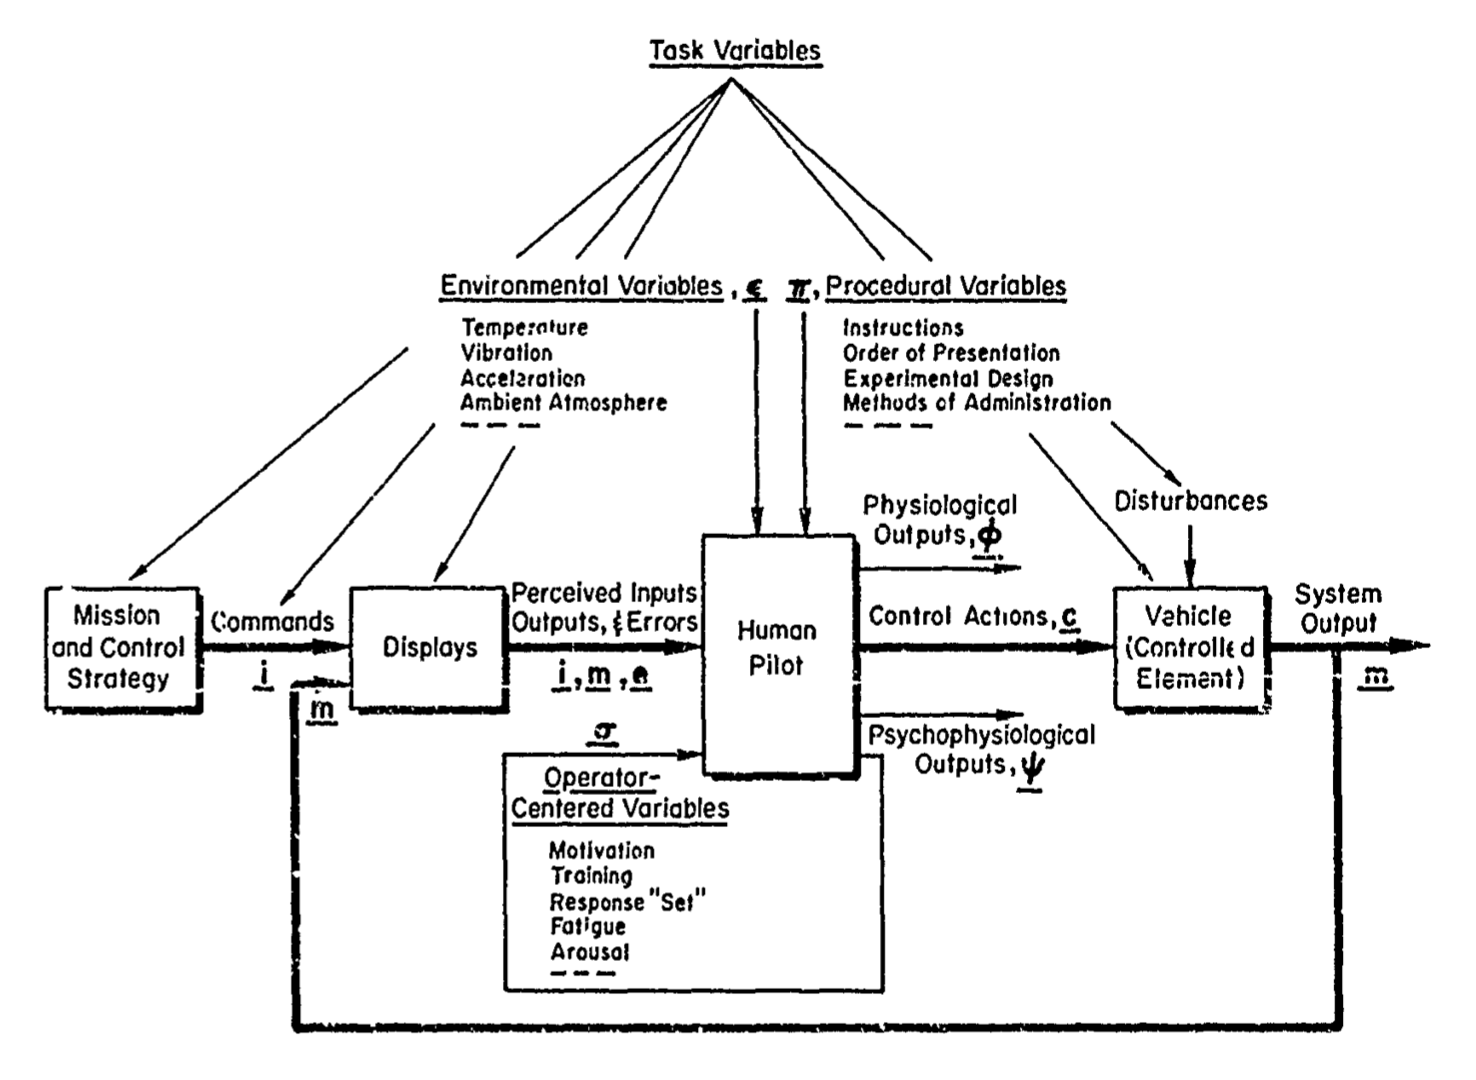
\includegraphics[width=0.8\linewidth]{figures/Introduction/Screen_Shot_2018-07-25_at_10_37_08_AM.png}
        \caption[Variables affecting the pilot/vehicle system]{Variables affecting the pilot/vehicle system, from~\citep{mcruer_mathematical_1974}.}
        \label{figure:mcruer1974}
    \end{center}
\end{figure}

In addition to popularizing the concept of feedback, the creation of control theory in the early 1940s also provided the tools required for the mathematical modeling of the human pilot.
At the time, new weapons were being created for World War 2 which could only be used effectively with trained operators working in tandem with the machine.
While it was thought that a human could be viewed as a unique kind of servomechanism in the control feedback loop, it was still unclear what factors affected human performance.
Early work by Tustin and others extended the control theory framework and applied these theories to actual human operators~\citep{tustin_investigation_nodate}.
Particular interest was focused on ``attempt[ing] to find the laws of relationship of movement and error. In particular, it was hoped that this relationship [would] be approximately linear and so permit well developed theory of `linear servomechanisms' to be applied to manual control in the same way as it applies to automatic following~\citep{tustin_investigation_nodate}.''
This would allow for the prediction of human performance and the ability to predict the limits of human control.

These early works were summarized in McRuer's 1957 report, ``Dynamic Response of Human Operators''~\citep{mcruer_dynamic_1957}.
This work evaluated measurements for single-input/single-output (SISO) manual control systems and developed predictive models consistent with this data.
Indeed, McRuer writes, ``[i]t is possible, without doing violence to the data, to obtain describing functions which are generally applicable to the results of the many diverse experiments~\citep{mcruer_dynamic_1957}.''
The report concludes by describing a hypothetical transfer function of the human operator which includes a time delay, a neuromuscular lag, and a gain.
McRuer's early model of the complete pilot/vehicle system is presented in Figure~\ref{figure:mcruer1974}.
McRuer revisited these results in 1974, after three decades of supporting engineering and experimental psychology experiments and was able to further generalize these results to a wide variety of system dynamics~\citep{mcruer_mathematical_1974}.
In his study, McRuer completed a detailed analysis which included the human response to proportional, rate/velocity, and acceleration type controlled element dynamics, see Table~\ref{table:mcruer1974a}.
The result of this report was the now famous ``crossover model,'' which relates the operator and controlled element transfer characteristics by the equation
\begin{align}
    Y_c(jw) Y_p(jw) = \dfrac{w_c e^{-jw \tau_e}}{jw}
\end{align}
where $Y_c$ is the controlled element transfer function, $Y_p$ is the approximate human operator transfer function, $w_c$ is the crossover frequency, and $\tau_e$ is the effective time delay of the pilot.
The crossover model is so named as it allows for linear behavior at approximately -20 dB/decade slope in the region of the crossover frequency.
The approximate human operator response to several controlled element transfer functions and their combined open-loop transfer function are presented in Table~\ref{table:mcruer1974b}.
Modeling the human pilot with the crossover enabled a more complete view of the complete pilot/vehicle system, and allowed for human factors recommendations towards the design of new vehicles.
Even today, the crossover model is used as the standard for describing pilot/vehicle systems at the crossover frequency~\citep{mcruer_human_1965, mcruer_mathematical_1974, xu_review_2017}.

\begin{table}[tb]
    \centering
    \includetable{intro-idealized-control-elements.tex}
    \caption[Example Applications of Idealized Controlled Element Forms]{Example Applications of Idealized Controlled Element Forms, adapted from~\citep{mcruer_mathematical_1974}.}
    \label{table:mcruer1974a}
\end{table}

\begin{table}[tb]
    \centering
    \includetable{intro-human-operator-characteristics.tex}
    \caption[Summary of Human Operator Approximate Characteristics]{Summary of Human Operator Approximate Characteristics, adapted from~\citep{mcruer_mathematical_1974}.}
    \label{table:mcruer1974b}
\end{table}

The continued demand for human pilot models for use in informing vehicle design, as well predicting, preventing, and explaining accidents has led to a variety of more complex pilot models since the creation of the crossover model.
A recent review by Xu et al. in 2017 surveyed the state of the art in human pilot modeling and grouped existing models into three classes of models based on: control theory, human physiology, and intelligence techniques~\citep{xu_review_2017}.
Classical models based on control theory include the McRuer crossover model and optimal control models by Kleinman et al. developed in the early 1970s~\citep{kleinman_optimal_1970, baron_optimal_1970}.
Of these three overarching sets of models, the models based on human physiology are of the greatest interest here.
Models based on human physiology were developed to understand human pilot perception and control behavior, and include the Hess structural model~\citep{hess_structural_1980, hess_model_1990, hess_unified_1997}, Hosman's descriptive model~\citep{hosman_pilots_nodate, hosman_pilots_1999}, and the biodynamic model~\citep{griffin_validation_2001}.
Recent intelligence models take advantage of techniques including fuzzy control and neural networks~\citep{zaychik_conspectus_2006, gestwa_modelling_2003}.

\begin{figure}[tb!]
    \begin{center}
        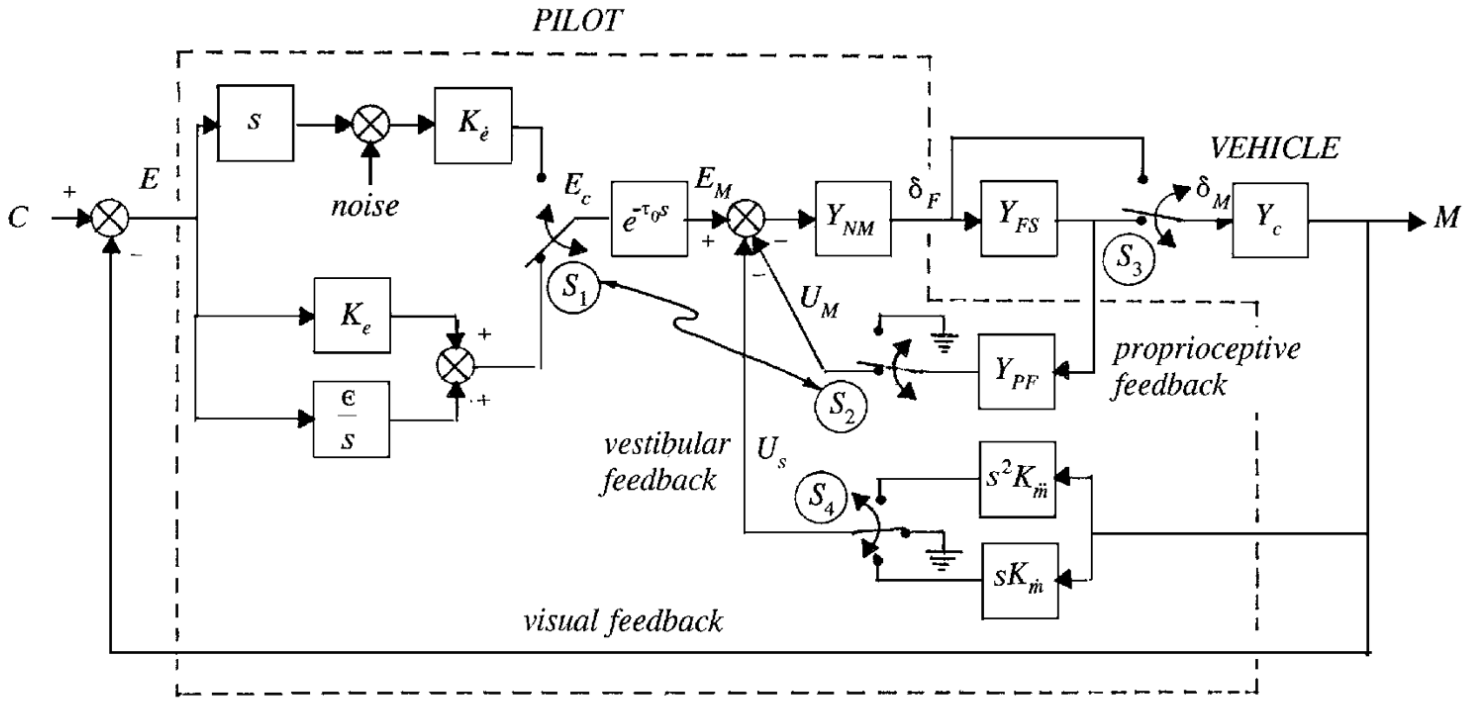
\includegraphics[width=0.8\linewidth]{figures/Introduction/Screen_Shot_2018-07-31_at_11_21_44_AM.png}
        \caption[The Hess Structural Model of the Human Pilot]{The Hess Structural Model of the Human Pilot, from~\citep{hess_unified_1997}.}
        \label{figure:structuralmodel}
    \end{center}
\end{figure}

While the McRuer was very successful in predicting pilot behavior, it it did not attempt ``to describe the underlying structure which contributes to human pilot dynamics~\citep{hess_structural_1980}.''
For this reason, the Hess Structural Model is of particular interest due to the incorporation of multiple sensory channels and models of visual acuity and the time-varying human pilot~\citep{hess_modeling_2009}.
The Structural Model includes the effects of the neuromuscular system, the force-feel characteristics of the input device, and the contributions of proprioceptive, vestibular, and visual feedback, see Figure~\ref{figure:structuralmodel}.
One of the key strengths of the Structural Model is the relatively few number of free parameters that need to be set to predict pilot performance.
The model has been used in predicting and evaluating handling qualities and pilot-induced oscillation rating levels for helicopters, Boeing 747, Lockheed C-5A, and twin ducted-fan aircraft~\citep{hess_analytical_2013, andreea-irina_prediction_2014, grant_handling_2015}.
Hess has also investigated how pilot control characteristics change with time due to flight anomalies, changing flight dynamics, and sudden increases in task demand~\citep{hess_modeling_2009, hess_modeling_2016}.
The results of this model have been compared to the results of a human-in-the-loop simulation for a well trained subject, and showed good comparison~\citep{hess_modeling_2016}.
Recent work from Bachelder et al. has included modifications to the Structural Model to link pilot performance and workload and to enable the modeling of pulsive pilot behavior~\citep{bachelder_modeling_2017, bachelder_linking_2018}.

\subsection{Summary}
We propose to run human-in-the-loop subject testing experiments to understand the effects of concurrent bandwidth feedback, and to integrate the effects of this feedback into a human performance model.
To investigate the two Aims outlined below, we completed four experiments and the development of a model.

\begin{description}[align=left]
    \item [Aim One] Investigate the effects of concurrent bandwidth feedback on human performance and workload effects in complex manual control task.
    \item [Aim Two] Extend the Hess Structural Model of the human pilot to include the effects of concurrent bandwidth feedback.
\end{description}

Concurrent bandwidth feedback has been used in a large variety of motor control tasks, and has generally been found to improve performance.
Until recently, however, only simple tasks such as physical movements or low-dimensional pursuit tasks have been investigated.
More recent works, including the lane-keeping task by de Groot et al., and our previous work with the SAFER task, have indicated that concurrent bandwidth feedback can also be quite effective for complex tasks.
Unlike simple tasks, in which the guidance hypothesis dominates when feedback is removed, there is some evidence that concurrent bandwidth feedback can be removed after training without a loss of performance.
The decrease in required learning time, improved performance, and decreased workload seen in the SAFER task show that concurrent bandwidth feedback may prove to be most useful very early in training when subjects are first exposed to complex, highly dynamic tasks.
As concurrent bandwidth feedback can improve performance without an increase in workload, it may prove a useful technique for training other complex manual control tasks.

There has been considerable improvement in the field of pilot modeling since McRuer's crossover model, especially with models that incorporate human physiology.
The Structural Model, in particular, has been very effective in predicting pilot performance, handling qualities, pilot-induced oscillation rating levels, and workload for a variety of system dynamics.
None of these pilot models, however, are able to include the effects of concurrent bandwidth feedback.
The performance improving effects of this feedback, seen throughout the literature, make this a compelling feature to be incorporated into a pilot model.

\section{Research Questions}
\label{sec:intro_questions}
We are interested in measuring, modeling, and predicting the effects of concurrent bandwidth feedback (CBF) on human performance in complex manual control tasks.
To this end, this proposed research includes two research aims.
These aims build on each other, starting with a compensatory tracking task, extending to surface electromyography and aircraft flight tasks, and finishing with a theoretical model.
\begin{description}[align=left]
    \item [Aim One] Investigate the effects of concurrent bandwidth feedback on human performance and workload effects in complex manual control task.
    \item [Aim Two] Extend the Hess Structural Model of the human pilot to include the effects of concurrent bandwidth feedback.
\end{description}

There are a number of research questions that we intend to answer by completing these aims, which include:
\begin{enumerate}
    \item Can concurrent bandwidth feedback improve performance of complex manual control tasks?
          \begin{enumerate}
              \item Can CBF reduce the required training time to peak performance?
              \item Can CBF be removed after reaching peak performance without reducing subject performance (i.e., does the guidance hypothesis not hold)?
              \item Does CBF improve performance in transfer of training tasks?
              \item Can performance be increased without increasing workload?
          \end{enumerate}
    \item Can we develop a model of human performance which includes the effects of concurrent bandwidth feedback?
          \begin{enumerate}
              \item Can we use this model to estimate operational limits?
          \end{enumerate}
\end{enumerate}

\section{Summary}
We have introduced our goals and motivation for the design and use of the concurrent bandwidth feedback, a techique for enhancing motor control training without inducing higher levels of workload.
The background for the experimental work has been described and the open research questions that we explore in this work have been summarized.
In the following chapters, we first present a systematic assessment of current and upcoming human automation/robotic integration technologies and research topics (Chapter~\ref{chapter:tradestudy}), then report on four experiments involving augmented feedback (Chapters~\ref{chap:3dtracking}-\ref{chapter:aircraftfeedback}), propose a theoretical model which explains the observed effects of the feedback (Chapter~\ref{chapter:modeling}), and summarize our findings and proposed future work (Chapter~\ref{chap:conclusion}).

\chapter{Conclusion}
\label{chap:conclusion}

\textbf{\color{red} This chapter does not yet exist.}

\section{Research Questions}

In Chapter~\ref{sec:intro_questions}, we listed seven research questions that we aimed to answer by this research.
Here we summarize our answers to these questions.

\section{Future Work}



% note that the 'plainnat' style does not allow URL's in the bibtex entry
%
% some ideas here:
% http://bib2web.djvuzone.org/bibtex.html
%

% reset the page style
%\pagestyle{plain}


% To enable this it will need to be added to toc so it's not in a chapter
\pagestyle{plain}

\ssp
\bibliography{dissertation}

% the appendix:
% there are several sections, that don't really fit into the main chapters
%
\part*{\addcontentsline{toc}{part}{Appendices}Appendices}
\appendix

% reset page style to fancy
%\pagestyle{fancyplain}

\chapter{Trade Analysis Tables} \label{appendix:trade-tables}

\begin{figure}[b!]
    \begin{center}
        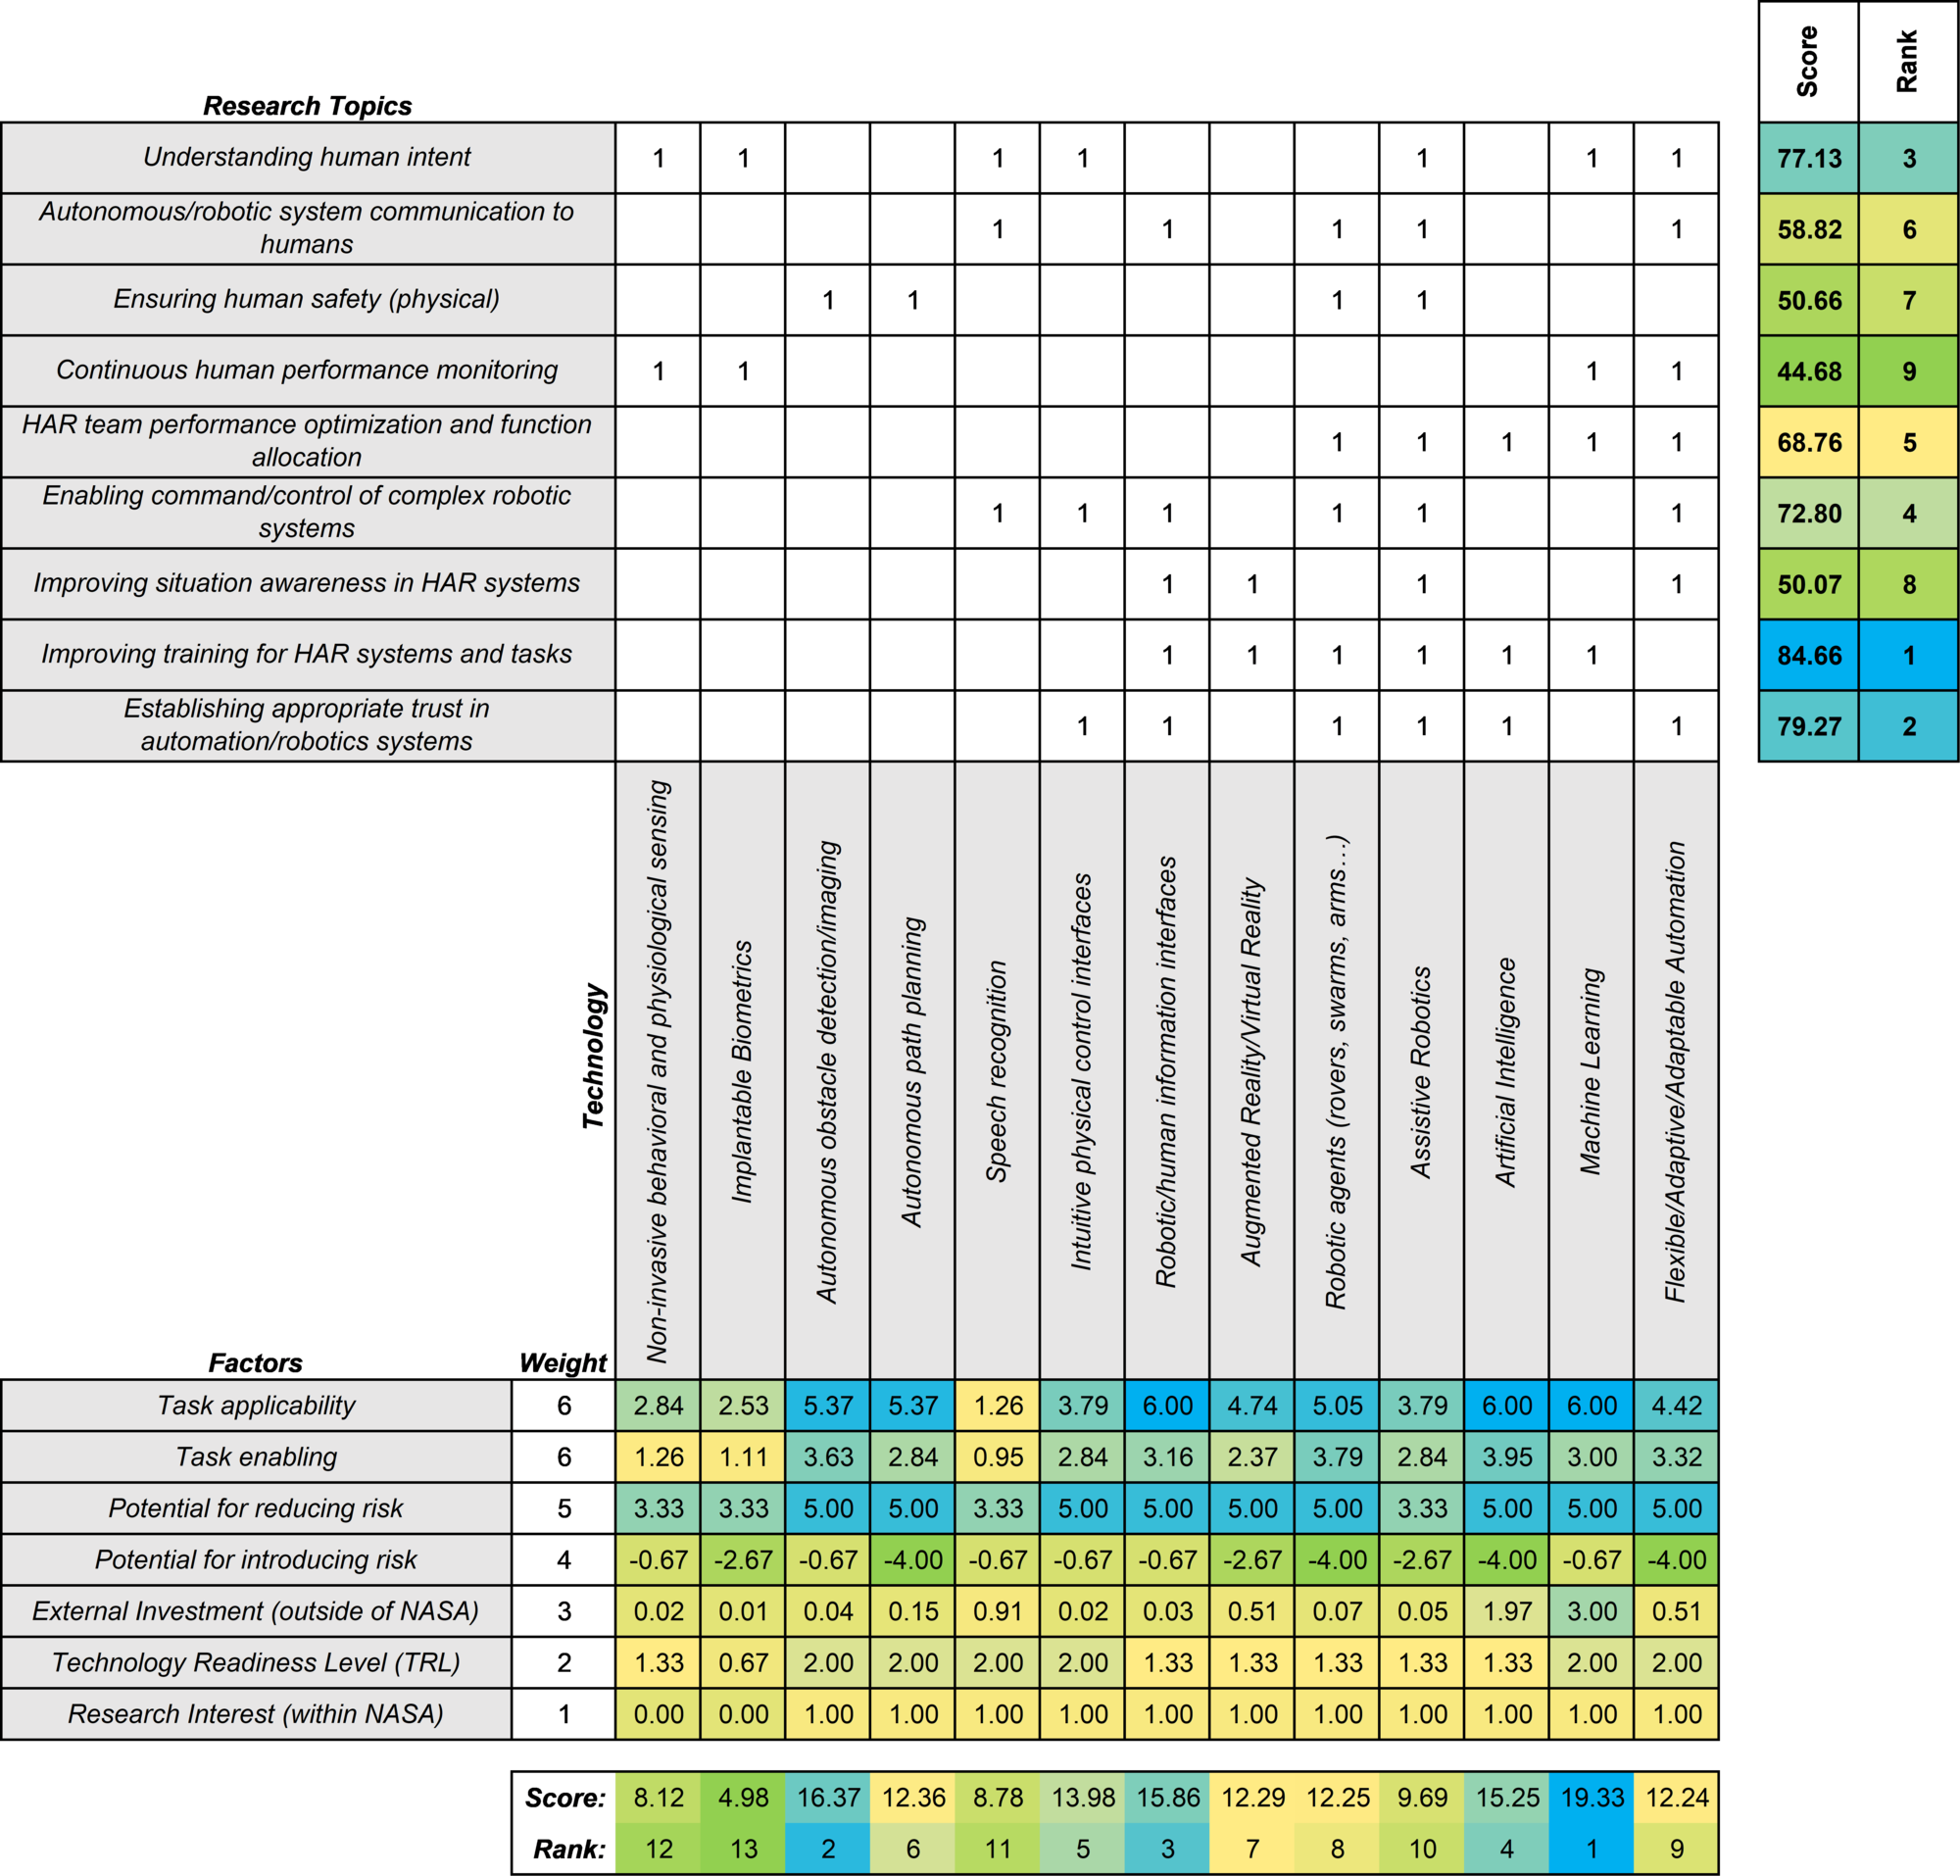
\includegraphics[width=0.8\linewidth]{figures/TradeStudy/figurea1.png}
        \caption[Top-level trade table]{Top-level trade table with final research topic scores (top right), final technology scores based on factors (bottom) and weighted factor-level scores for each technology.}
        % \label{figure:}
    \end{center}
\end{figure}

\begin{figure}[b!]
    \begin{center}
        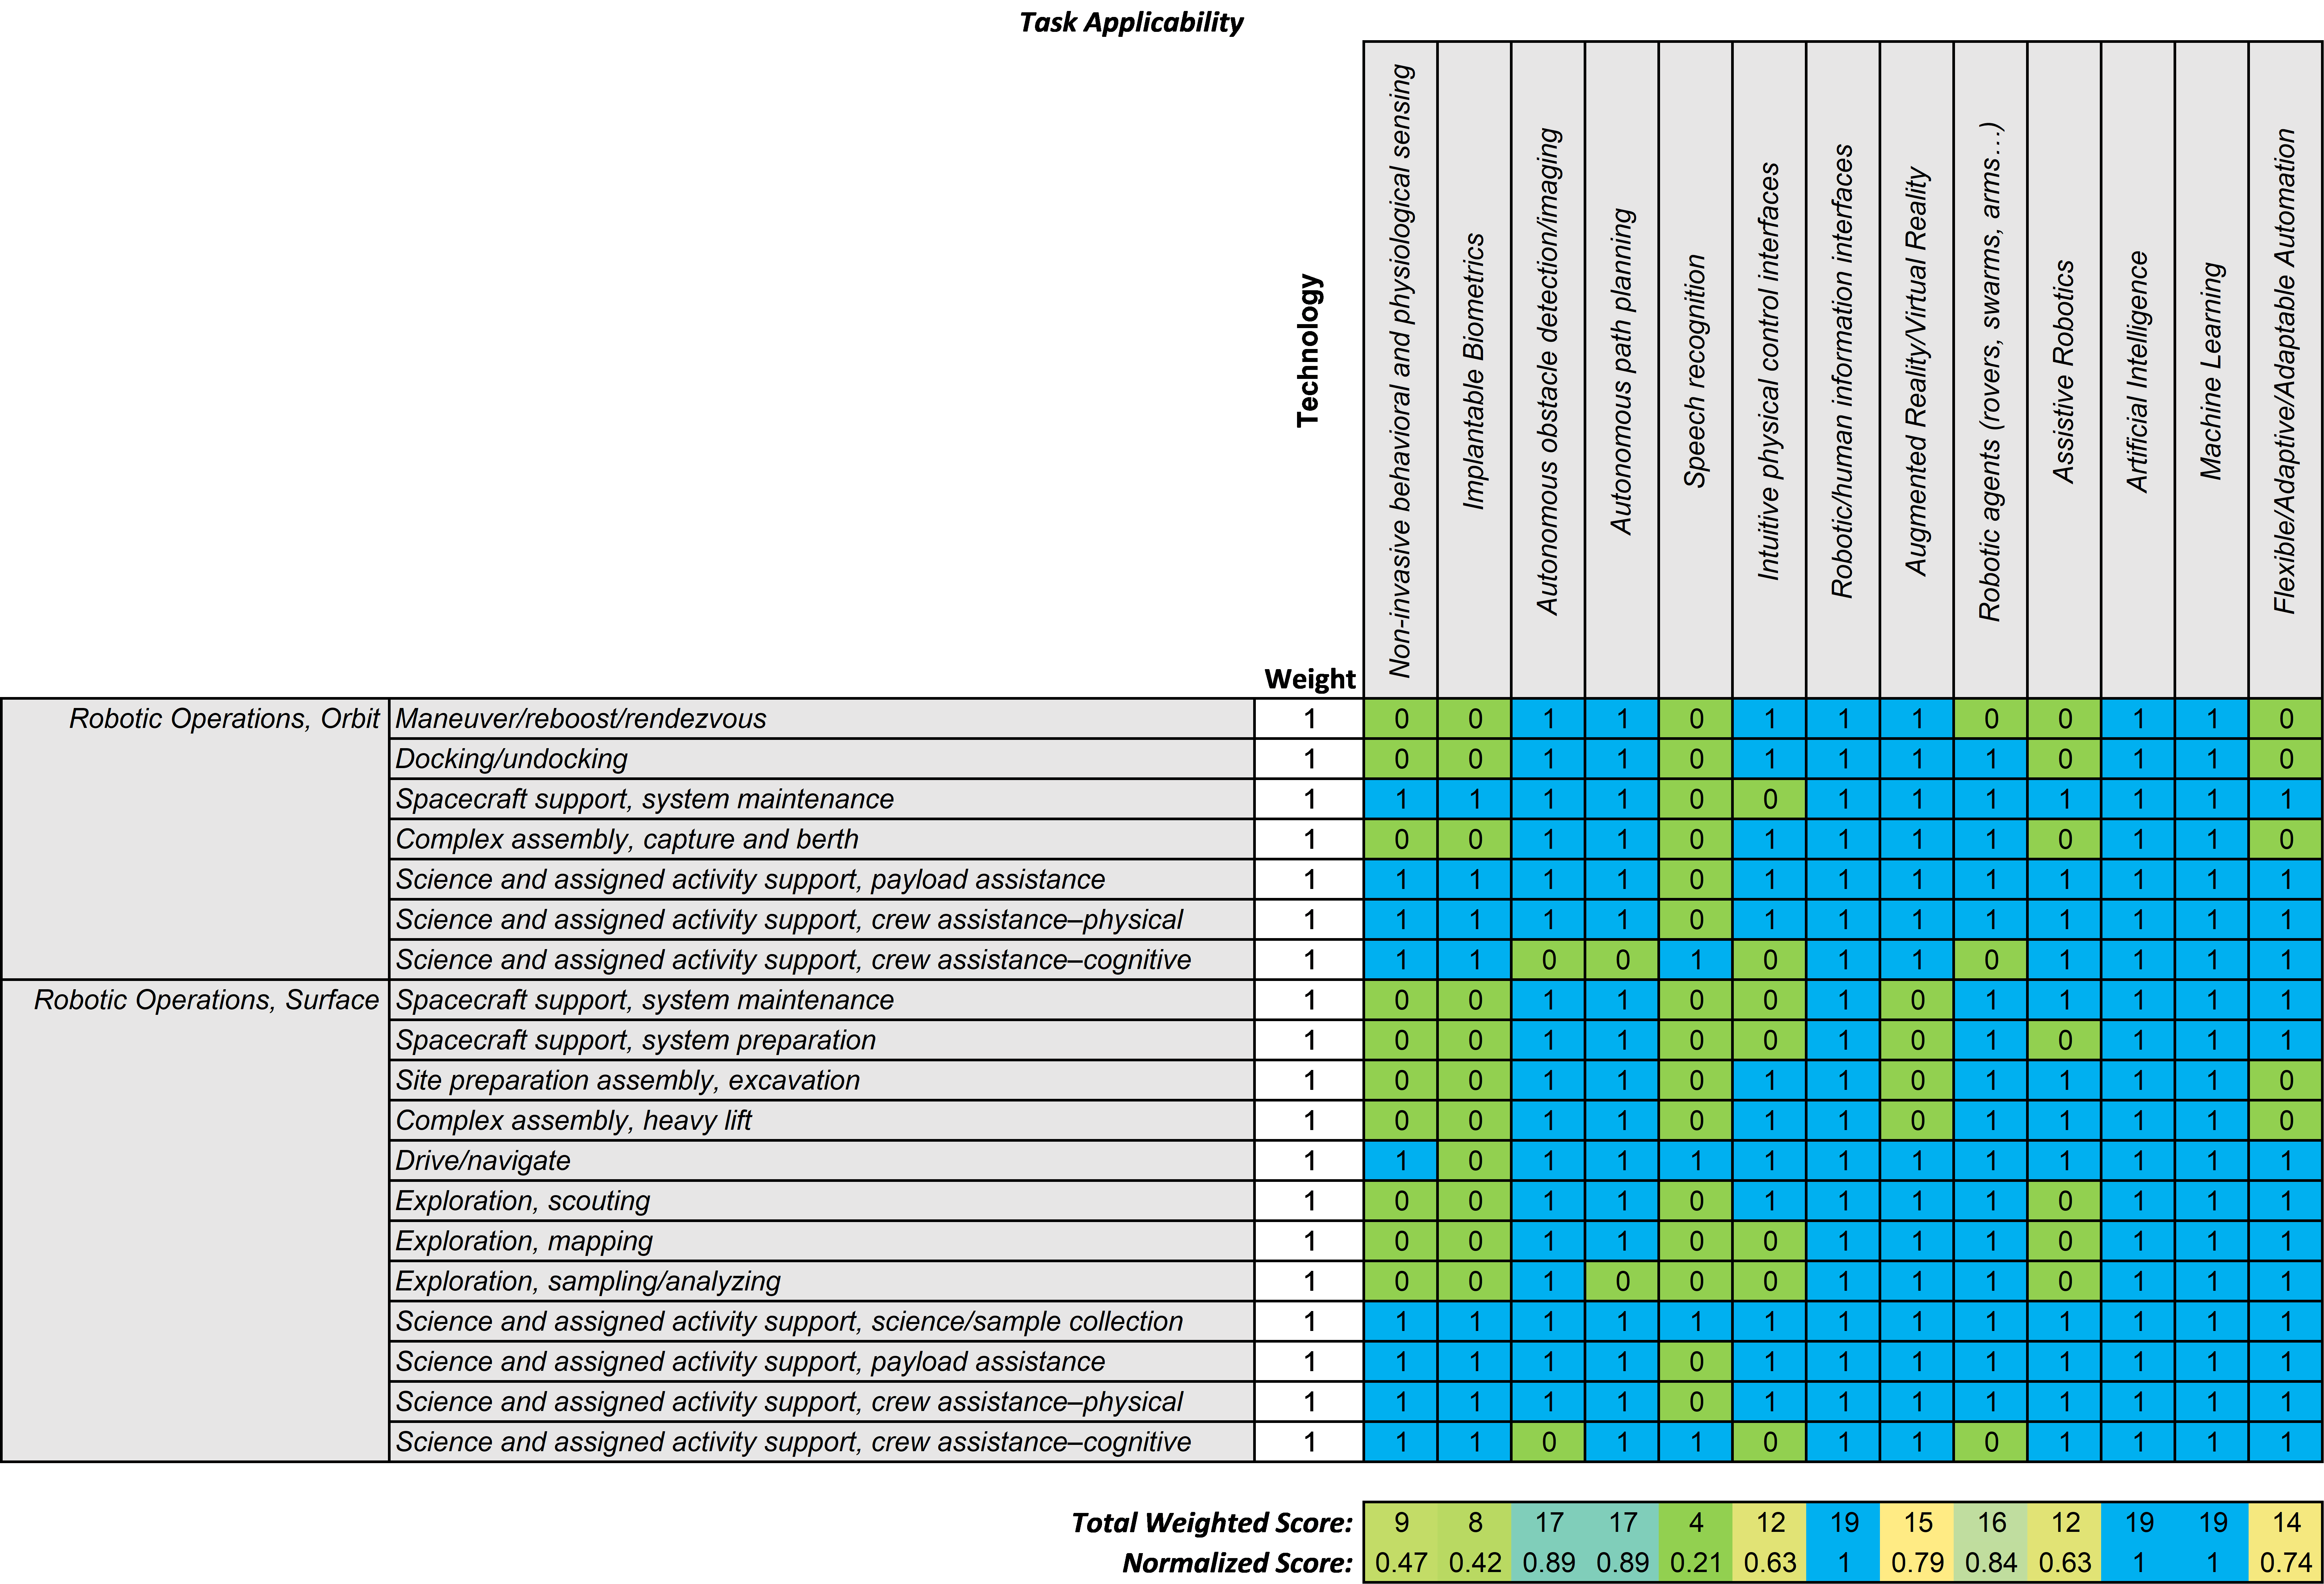
\includegraphics[width=0.8\linewidth]{figures/TradeStudy/figurea2.png}
        \caption[Technology to Task Applicability factor-level trade table]{Technology to Task Applicability factor-level trade table.}
        % \label{figure:}
    \end{center}
\end{figure}

\begin{figure}[b!]
    \begin{center}
        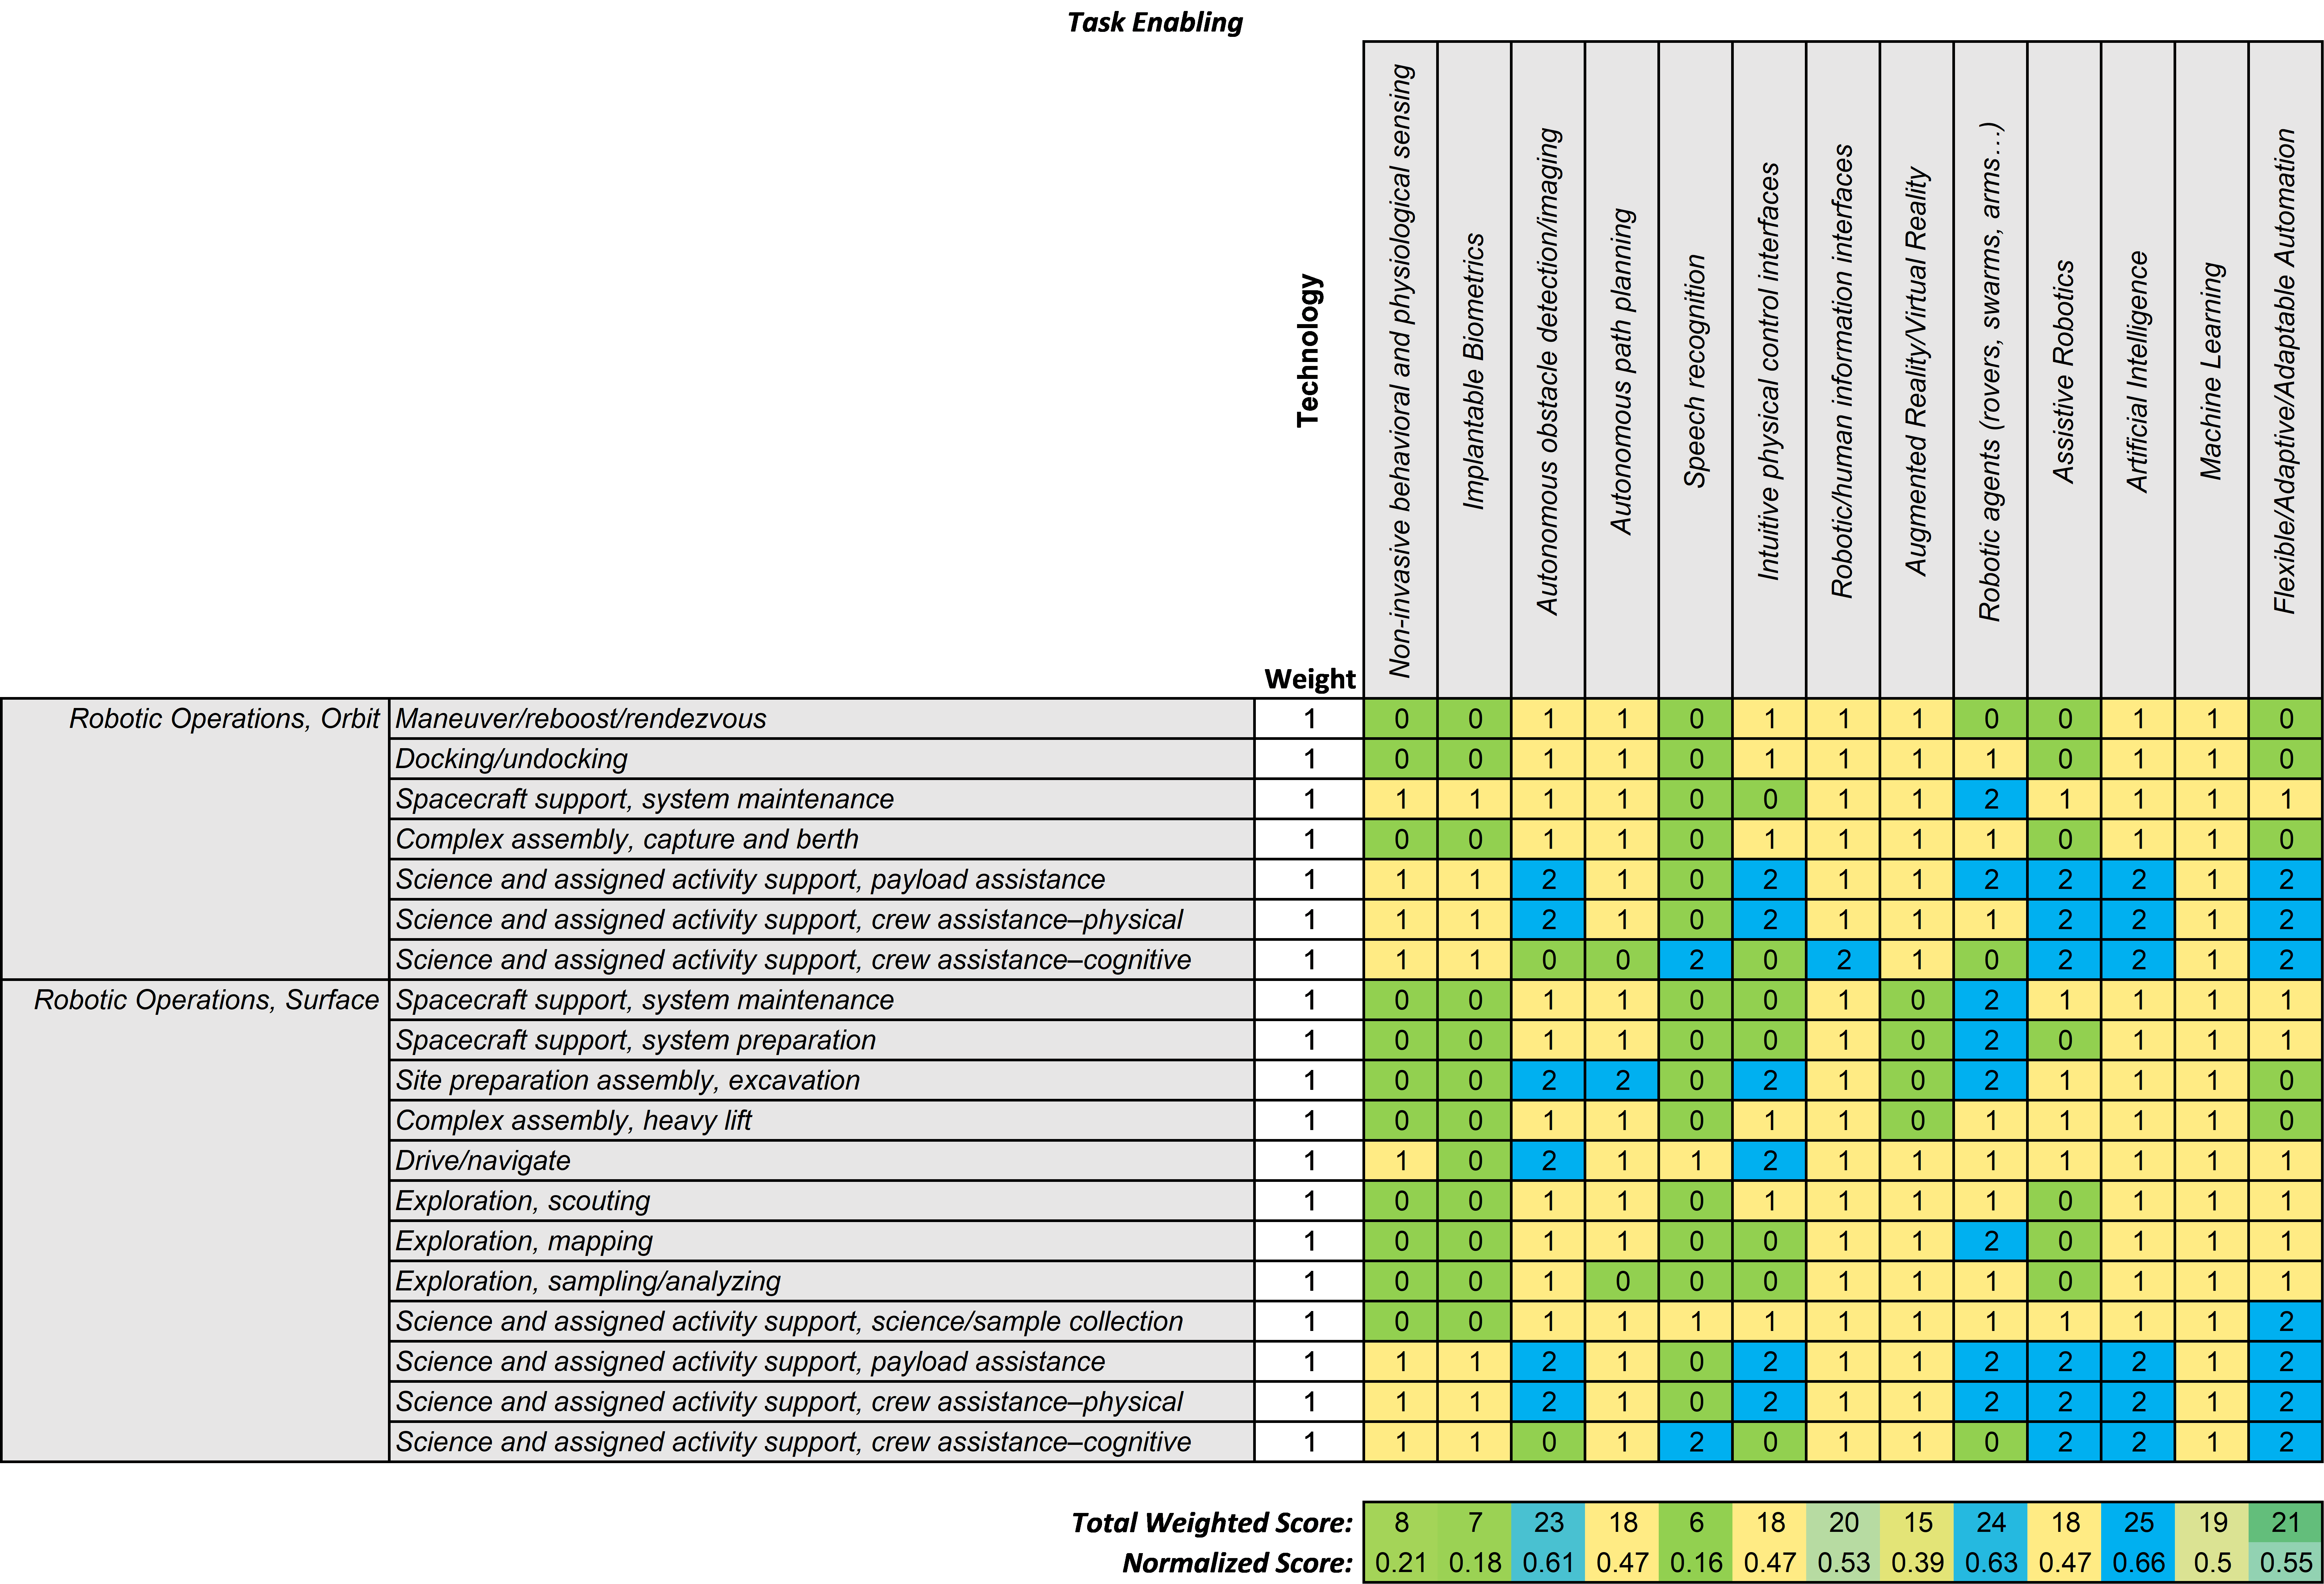
\includegraphics[width=0.8\linewidth]{figures/TradeStudy/figurea3.png}
        \caption[Technology to Task Enabling factor-level trade table]{Technology to Task Enabling factor-level trade table.}
        % \label{figure:}
    \end{center}
\end{figure}

\begin{figure}[b!]
    \begin{center}
        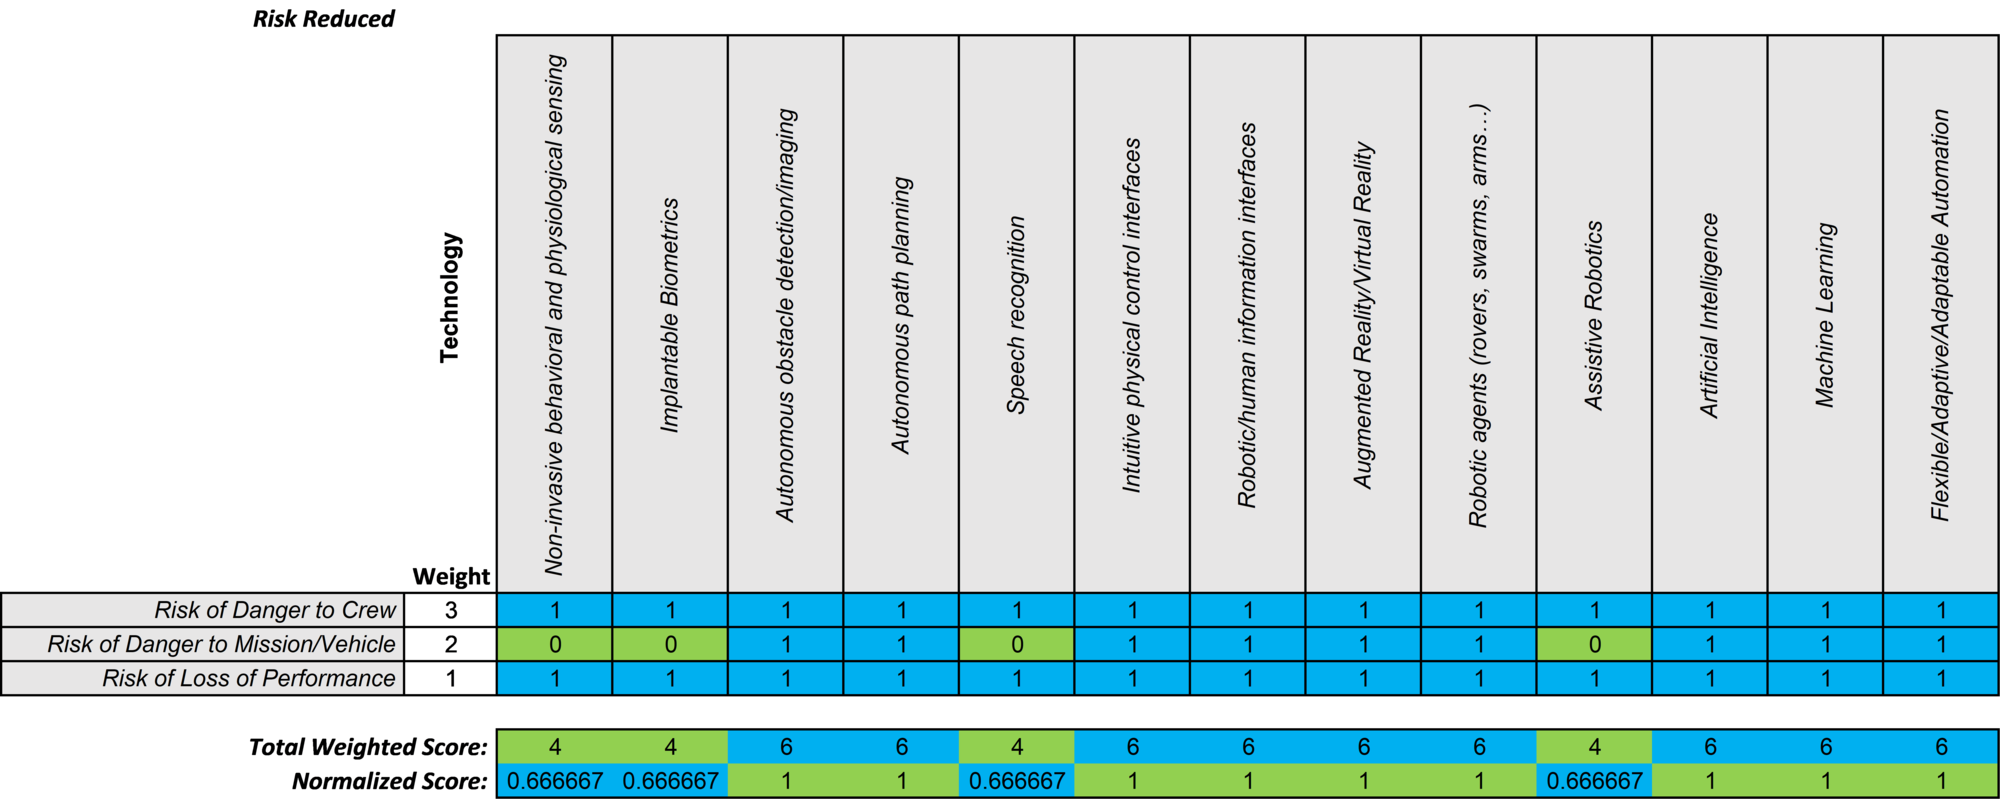
\includegraphics[width=0.8\linewidth]{figures/TradeStudy/figurea4.png}
        \caption[Technology to Risk Reduced factor-level trade table]{Technology to Risk Reduced factor-level trade table.}
        % \label{figure:}
    \end{center}
\end{figure}

\begin{figure}[b!]
    \begin{center}
        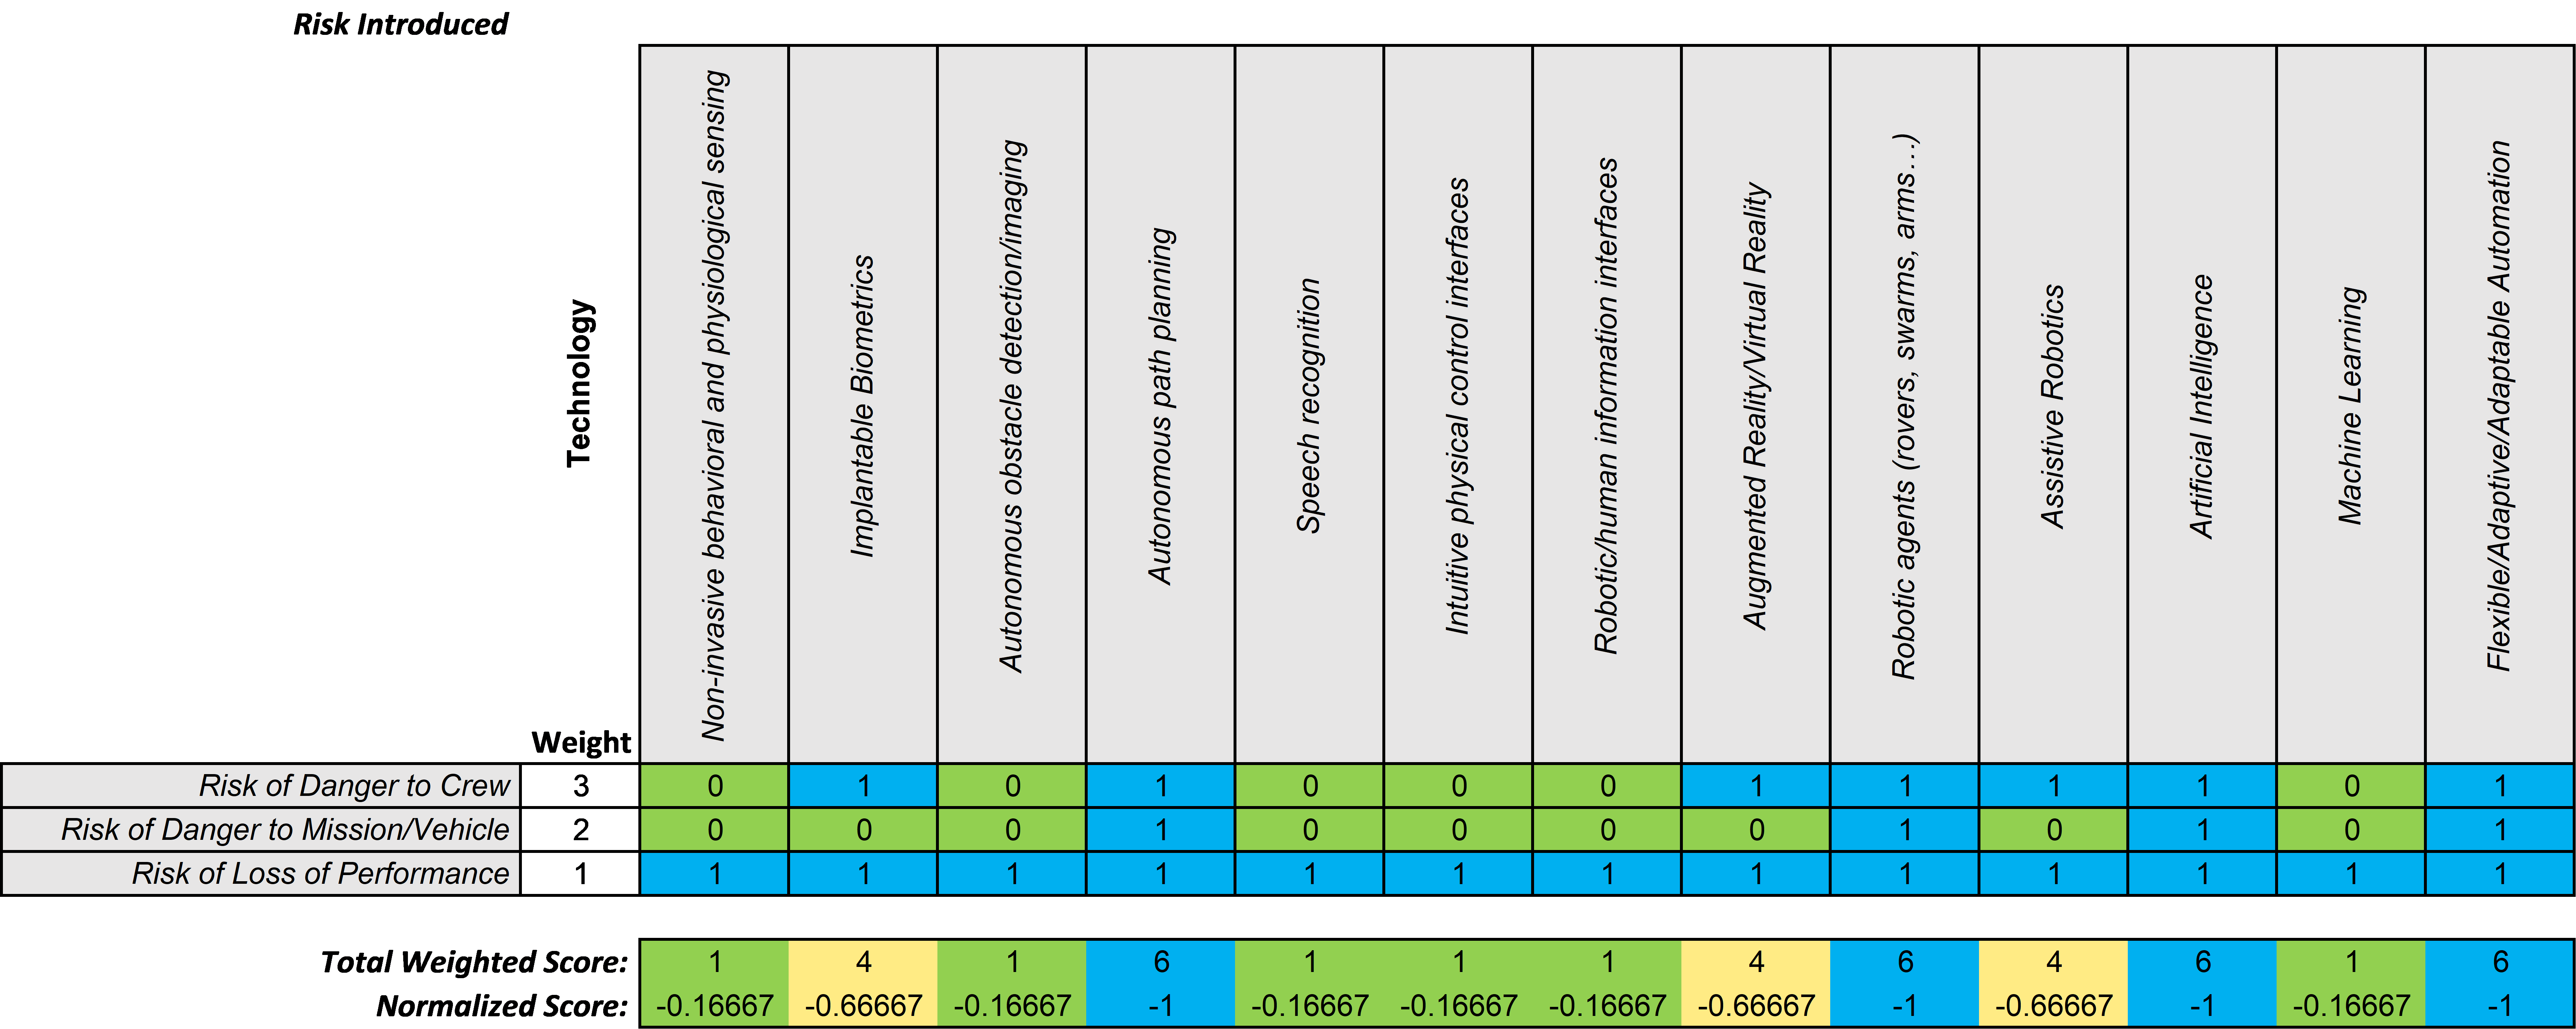
\includegraphics[width=0.8\linewidth]{figures/TradeStudy/figurea5.png}
        \caption[Technology to Risk Introduced factor-level trade table]{Technology to Risk Introduced factor-level trade table.}
        % \label{figure:}
    \end{center}
\end{figure}

\begin{figure}[b!]
    \begin{center}
        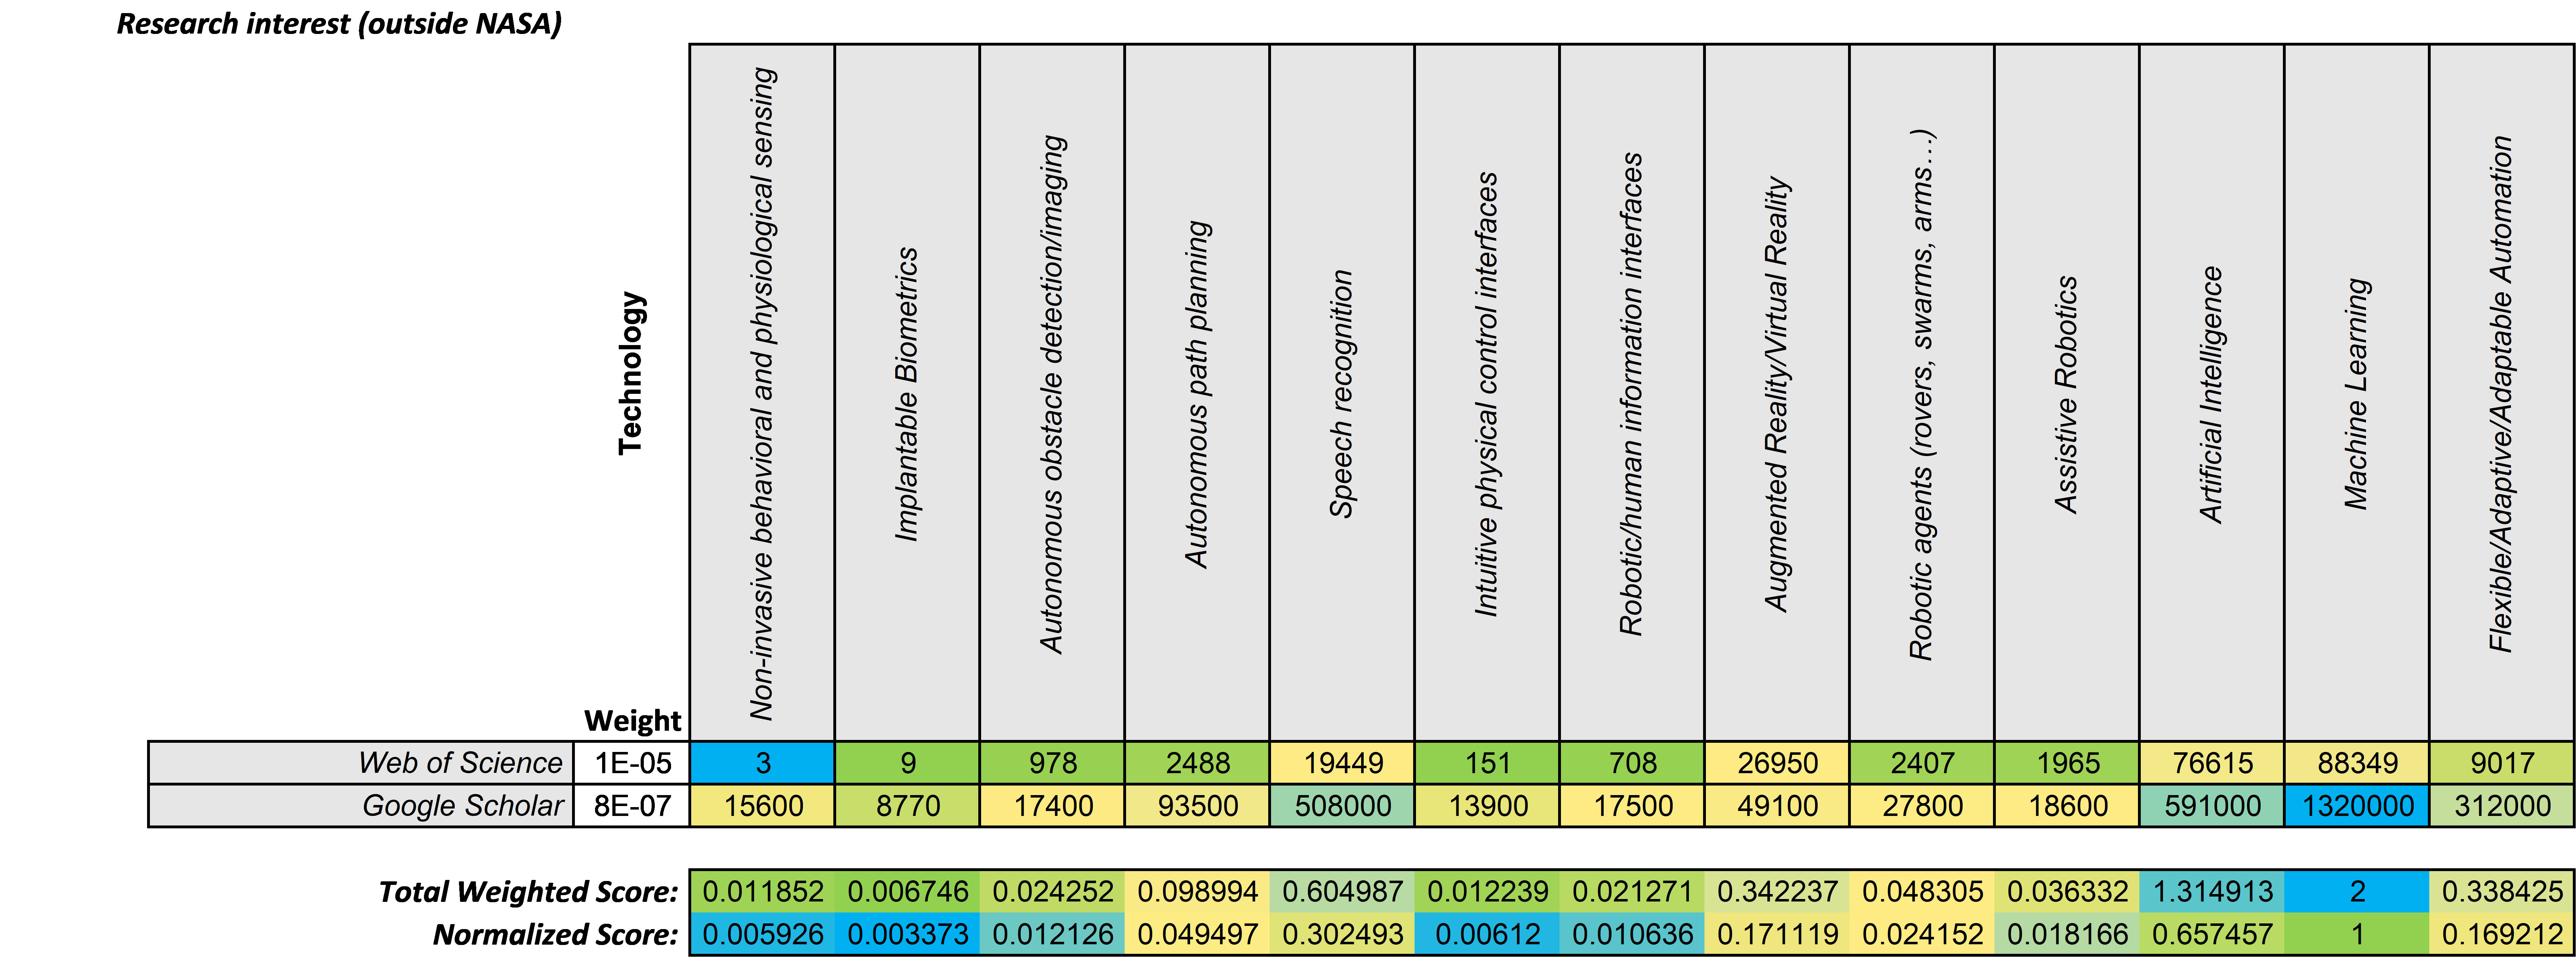
\includegraphics[width=0.8\linewidth]{figures/TradeStudy/figurea6.png}
        \caption[Technology to Research Interest (outside NASA) factor-level trade table]{Technology to Research Interest (outside NASA) factor-level trade table.}
        % \label{figure:}
    \end{center}
\end{figure}

\begin{figure}[b!]
    \begin{center}
        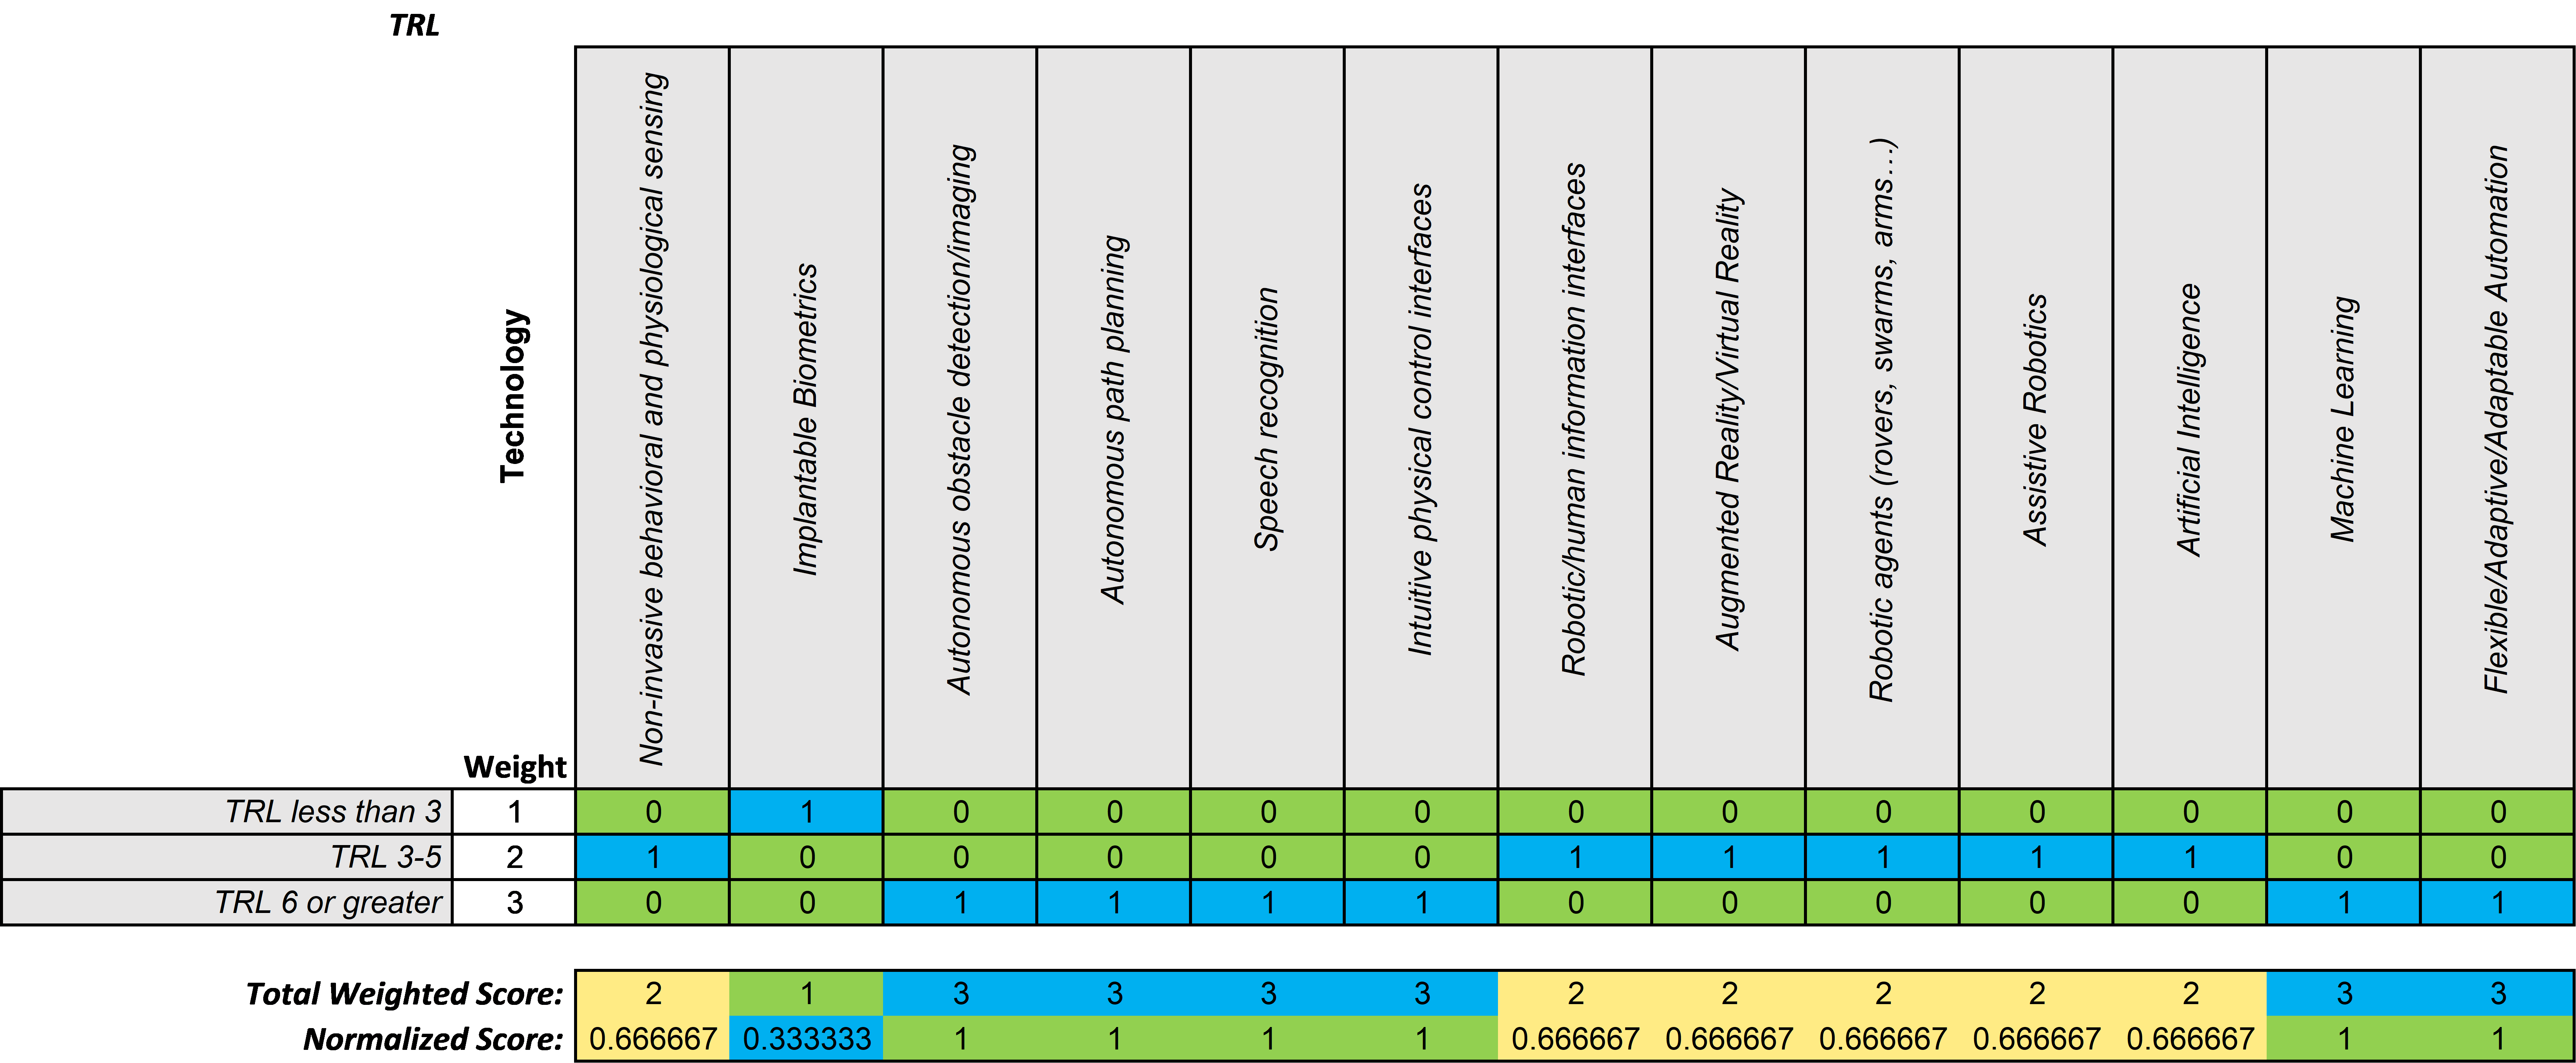
\includegraphics[width=0.8\linewidth]{figures/TradeStudy/figurea7.png}
        \caption[Technology to TRL factor-level trade table]{Technology to TRL factor-level trade table.}
        % \label{figure:}
    \end{center}
\end{figure}

\begin{figure}[b!]
    \begin{center}
        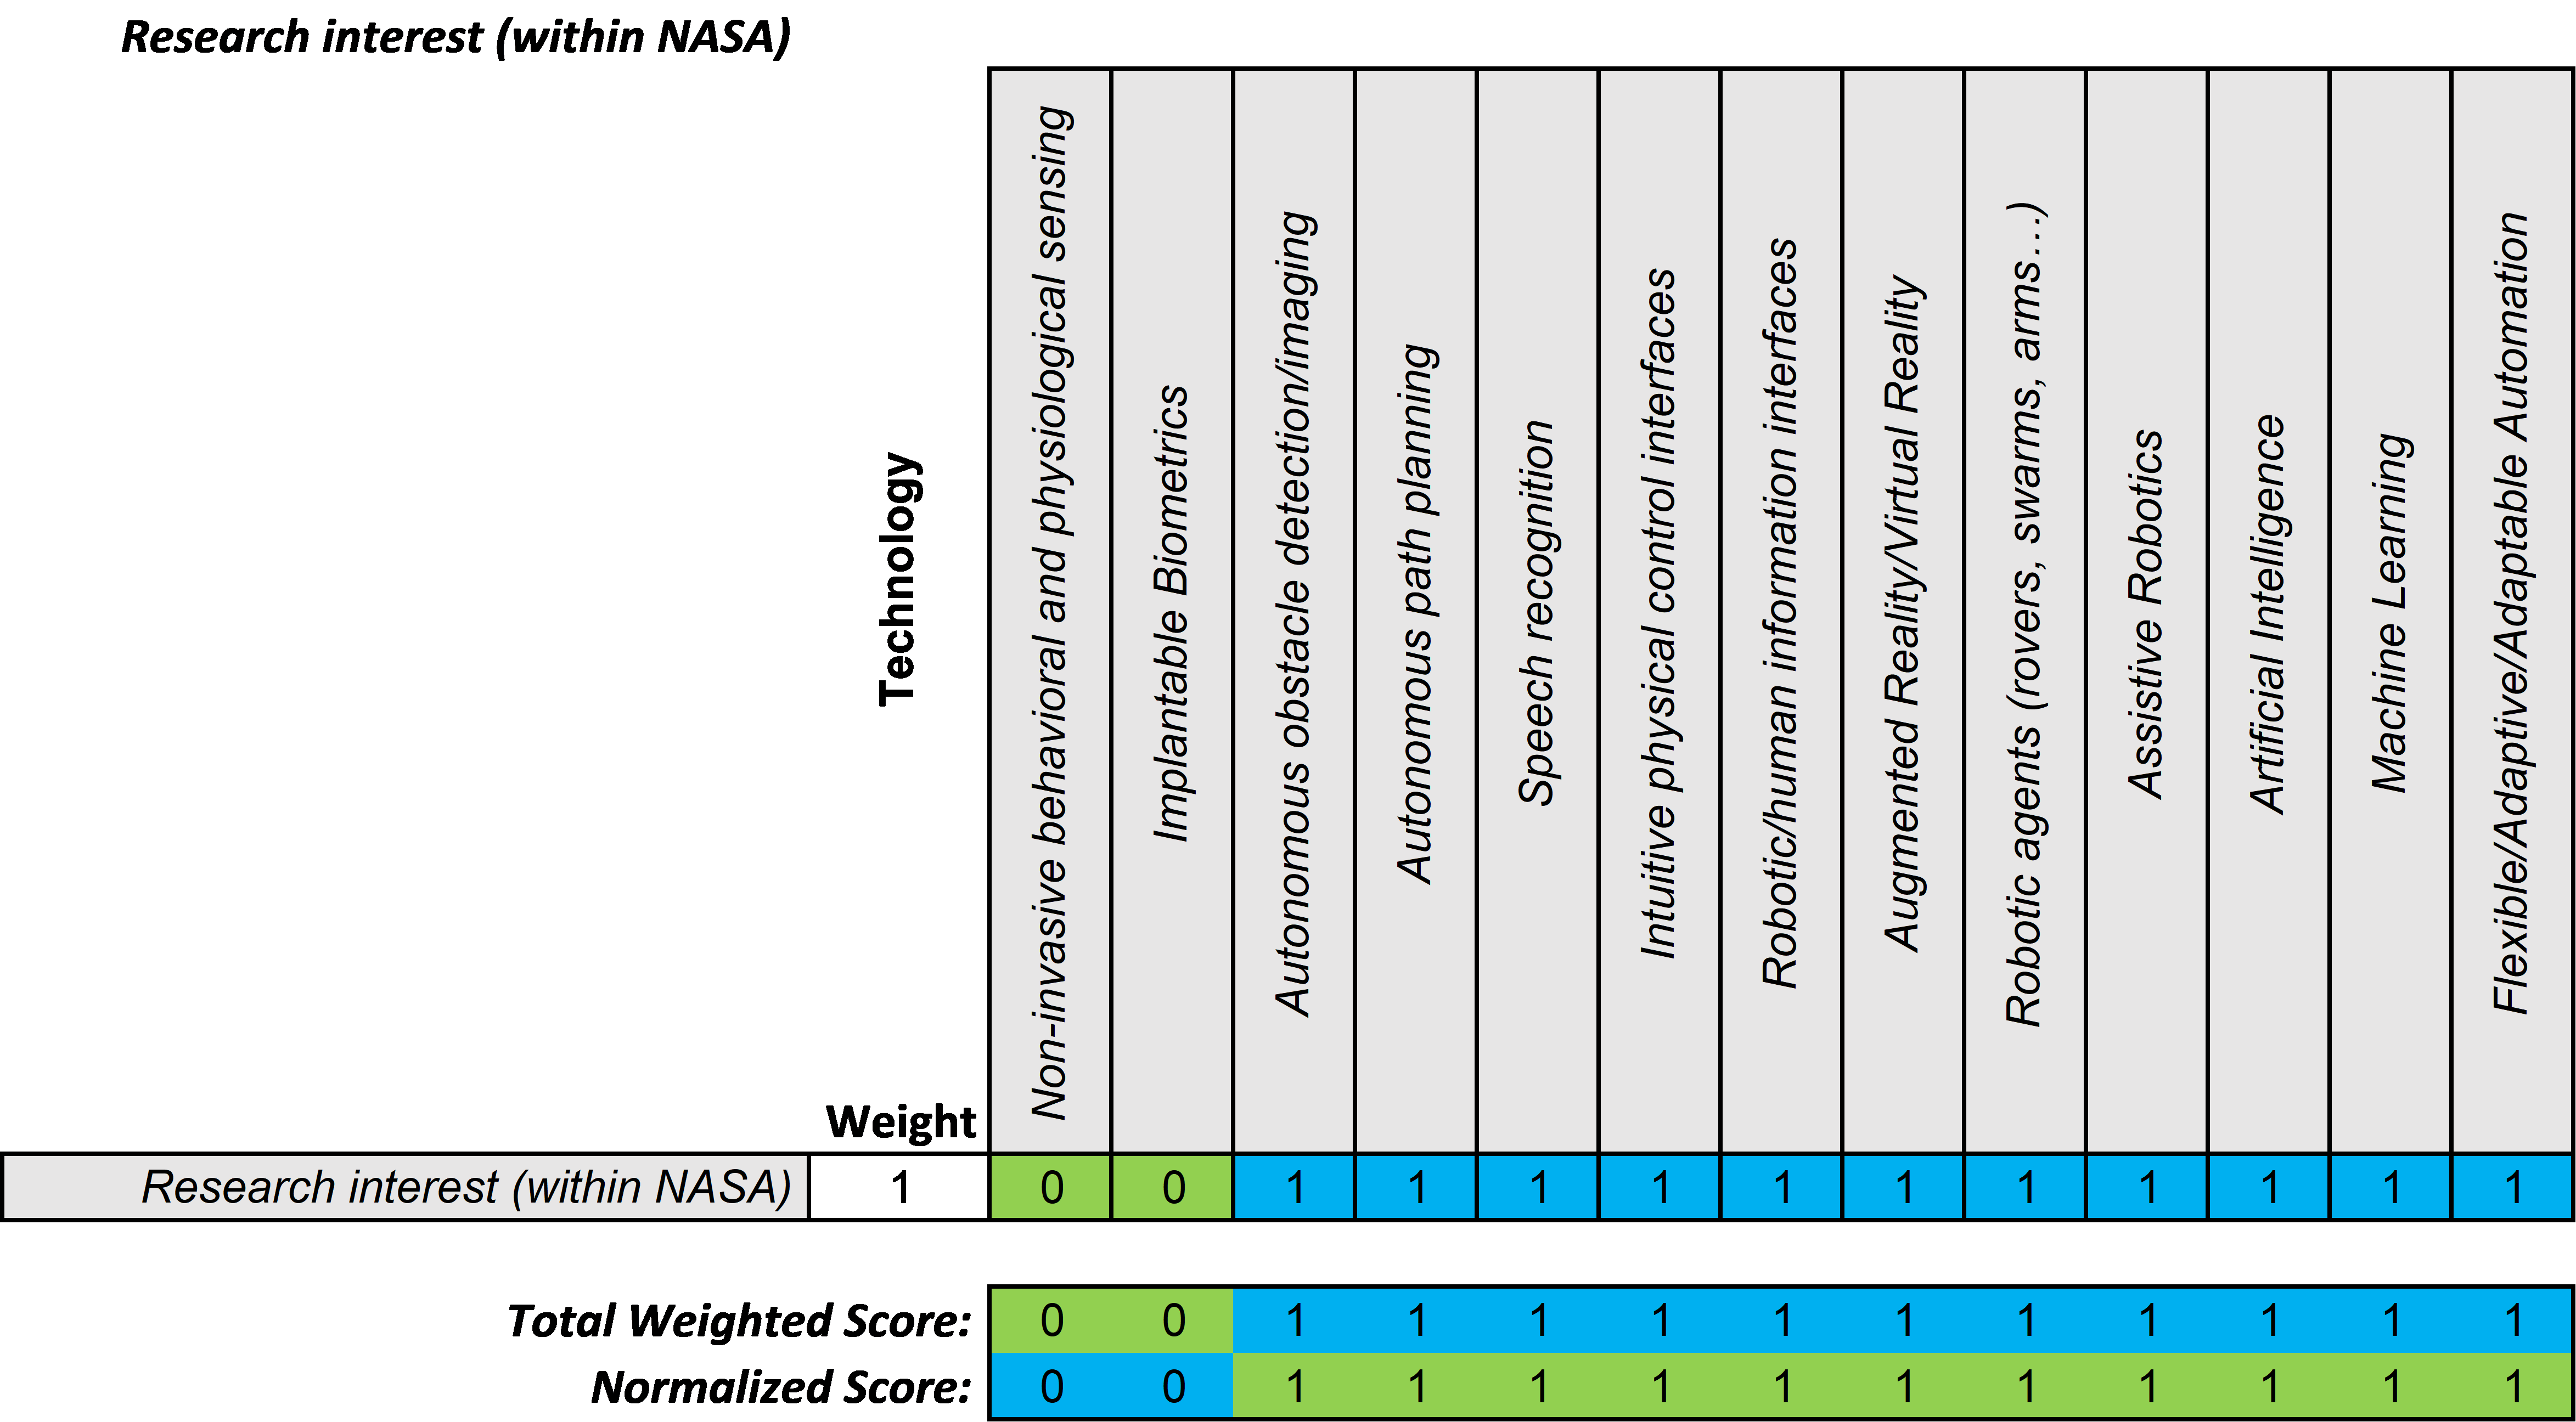
\includegraphics[width=0.8\linewidth]{figures/TradeStudy/figurea8.png}
        \caption[Technology to Research Interest (within NASA) factor-level trade table]{Technology to Research Interest (within NASA) factor-level trade table.}
        % \label{figure:}
    \end{center}
\end{figure}

% Appendix B: Subject Matter Expert Summary of Backgrounds
% The SMEs interviewed to gather background information on the HARI trade space all have extensive experience in either HAR integration research, human factors, or both, in their respective fields. Additionally, three SMEs have experience in related fields: one person in data analytics, and two others in psychology/neuroscience. The SMEs have a wide range of experience addressing different research applications, captured in Table B1.

% SME	Background	Expertise
% 		Space	Aviation	Military	Medical	Automotive	Locomotive	Robotics (general)
% 1	Industry		x	x
% 2	Industry		x	x
% 3	Academia	x	x			x	x	x
% 4	Industry,
% Former NASA	x	x		x
% 5	Military			x	x			x
% 6	Academia, Industry				x	x
% 7	Academia	x	x	x			x
% 8	Academia,
% Industry		x					x
% 9	Academia	x			x			x
% 10	Industry,
% Former NASA	x			x	x
% Table B1: Background and application area expertise of interviewed subject matter experts

% Appendix C: Annotated Bibliography
% Parasuraman, Raja, and Christopher D. Wickens. "Humans: Still vital after all these years of automation." Human factors 50.3 (2008): 511-520.
% 	In their 2008 review, Parasuraman and Wickens discuss major discoveries and developments in levels and stages of automation, reliance on and compliance with automation, and adaptive automation. "Parasuraman, Sheridan, and Wickens (2000) accordingly proposed an extension of the LOA concept to four information-processing stages: (a) information acquisition, (b) information analysis, (c) decision making, and (d) action, with each stage having its own LOA scale (for similar scales, see Endsley & Kaber, 1999; Endsley & Kiris, 1995)."
% Ososky, Scott, et al. "Building Appropriate Trust in Human-Robot Teams." AAAI Spring Symposium: Trust and Autonomous Systems. 2013.
% 	In their 2013 paper, Ososky et al. describe autonomous, intelligent robots as teammates, rather than tools, and describe the importance of appropriate, rather than maximal, trust in the human-robot team. They discuss how human operators must create a sufficiently developed mental model of a robot to appropriately use it for tasks which the robot can perform superiorly to the human. They note that inaccurate mental models can create "pitfalls for robotic system misuse or disuse", and that accurate mental models are required for the human to appropriately trust the robot. They argue that appropriate trust in the robotic system leads to how the robotic system is ultimately used.
% Beer, Jenay M., Arthur D. Fisk, and Wendy A. Rogers. "Toward a framework for levels of robot autonomy in human-robot interaction." Journal of Human-Robot Interaction 3.2 (2014): 74-99.
% 	In their 2014 paper, Beer, Fisk, and Rogers outline a framework for levels of robot autonomy (LORA) for human-robot interaction (HRI), with the goal of allowing researchers to identify the impacts of autonomy on the interaction between human and robot. They outline a set of guidelines which can serve as "(1) a set of guidelines suggesting task and environmental influences on robot autonomy, (2) guidelines for determining or measuring autonomy, (3) a taxonomy for categorizing autonomy, and finally, (4) a set of HRI variables that may be influenced by robot autonomy."
% Chen, Jessie YC, and Michael J. Barnes. "Human–agent teaming for multirobot control: A review of human factors issues." IEEE Transactions on Human-Machine Systems 44.1 (2014): 13-29.
% 	In their 2014 paper, Chen and Barnes identified important human factors issued related to human-agent teams in multirobot control. They conclude that agents acting as interfaces between human operators and intelligent systems are an efficient way for operators to supervise multiple systems, while natural language processing is not required, the agents must have the ability to recognize operator intent, and that mixed initiative architectures can take advantage of both the human's expertise and the agent's precision and ability to act quickly. Mixed initiative systems, a subset of flexible automation, which allows for a dynamic level of automation based on the operator's state and events in the environment. Chen and Barnes further note the importance of transparency in effectively calibrating operator trust in an autonomous system.
% Kehoe, Ben, et al. "A survey of research on cloud robotics and automation." IEEE Trans. Automation Science and Engineering 12.2 (2015): 398-409.
% 	Kehoe et al.'s 2015 paper considers robots and automation systems that rely on externally networked support, and focuses on the benefits of the cloud, including: big data, cloud computing, collective robot learning, and human computation. They note the state of the art in each of these areas while considering the current challenges and future directions research must should be taken. New issues associated with the rise in cloud technology include the need for techniques to consider time varying latency and quality of service, privacy concerns, and big data cleaning and filtering techniques. The note three levels at which a cloud computing framework are currently established: Infrastructure as a Service (IaaS), where bare operating systems are available; Platform as a Service (PaaS), where more structure is provided, including access to application frameworks, databases, and programming languages; and Software as a Service (SaaS), where software is made available online rather than as a local service. They conclude by proposing a fourth cloud framework, Robotics and Automation as a Service (RAaaS), which merges PaaS and SaaS frameworks to provide a cloud service which processes inputs for robotics, suggests output actions, and monitors results to update future recommendations.
% Rautaray, Siddharth S., and Anupam Agrawal. "Vision based hand gesture recognition for human computer interaction: a survey." Artificial Intelligence Review 43.1 (2015): 1-54.
% 	Rautaray and Agrawal's 2015 survey provides a summary of progress in the field of vision-based hand gesture recognition and reviews the three main phases of hand gesture recognition: detection, tracking, and recognition. They analyze existing literature and note the required advances to further improve hand gesture recognition systems. They note the primary application domains of hand gesture recognition are desktop applications, followed by gaming and sign language. In terms of the challenges of operating in real-time and robustness, the authors find that comparisons are difficult as there is no commonly accepted baseline technique to compare to. Psychological aspects of gestures have been found to play an important role in hand gesture recognition systems. The authors find that, despite plenty of research into the field, 3D based gesture representations are still less preferred to appearance-based hand gesture representations.
% Ruhland, Kerstin, et al. "A review of eye gaze in virtual agents, social robotics and hci: Behaviour generation, user interaction and perception." Computer Graphics Forum. Vol. 34. No. 6. 2015.
% 	Ruhland et al.'s 2015 review covers the state of the art in generating artificial entities which include attempts to replicate the human eye, the role of social robotics, and the human-computer interaction issues involved. They found that research into eye-gaze models would greatly benefit from a fundamental foundation, and that individual differences in eye gaze are often ignored as research has traditionally attempted to model and recreate general behavior. Human-robot interaction in the field of eye gaze has largely focused on shared attention and gaze cueing, factors that have affected task performance and user speech. The authors note several challenges mapping virtual to physical robots, especially that robot expression has fewer degrees of freedom. They also, however, suggest that physical systems may be able to better direct human gaze to targets of interest in a real environment as they can avoid the Mona Lisa gaze effect associated with virtual agents.
% Yanco, Holly A., et al. "Analysis of human‐robot interaction at the darpa robotics challenge trials." Journal of Field Robotics 32.3 (2015): 420-444.
% 	Yanco et al.'s 2015 paper reviewed team performance at the DARPA Robotics Challenge (DRC) trials, analyzing the results, team structure, and human-robotic interfaces. The DRC trials were designed to test humanoid robots' ability to respond to disaster scenarios where communications bandwidth was limited or degraded. Yanco et al.'s team analyzed 8 of the 15 teams which volunteered to participate in their study, observing their team interaction and robot's performance during the challenge. They identified four areas required for teams to be successful in the challenge: robot mobility, robot manipulation, situation awareness of the robot and its surroundings, and an effective way to command the robot. They further found that the most effective team was successful largely due to their: increased sensor fusion, which reduced the operator's cognitive load and reduced the need to repeat tasks; decreased number of operators, which both increased situational awareness and decreased the amount of required operator input.
% Kolling, Andreas, et al. "Human interaction with robot swarms: A survey." IEEE Transactions on Human-Machine Systems 46.1 (2016): 9-26.
% 	Kolling et al.'s 2016 review is the first survey of human-swarm interaction, and presents the basics of swarm robotics, the cognitive needs of a swarm operator, and the challenges involved with providing a human-swarm interface. They break the cognitive complexity of the human-robot system into three difficulties, using an analogy of computational complexity: robots performing independent activities, with complexity O(n), which allows more robots to be controlled simply by adding more operators in a linear manner; robots interacting with other robots fully autonomously, with complexity O(1), which allows for a fixed number of robots to control any number of robots; and the case where robot-robot interaction must be controlled by an operator, with complexity O(>n), as the dependencies between robots results in more demand faster than the number of robots grows. Under the assumption that O(1) complexity (only one operator) is desired, they review various control methods of conveying operator intent to the swarm.
% Phillips, Elizabeth, et al. "Human-animal teams as an analog for future human-robot teams: influencing design and fostering trust." Journal of Human-Robot Interaction 5.1 (2016): 100-125.
% 	In their 2016 paper, Phillips et al. discuss the advantages of human-animal teams as an analog for the ongoing development of human-robot teams. They discuss the ways that trust is established and changes in human-animal teaming, how these effects are beginning to be seen in human-robot teams, and how this trust determines how humans interact with their robotic teammates. They argue that including nonverbal communication in robots can help humans to better understand their actions and intents, allowing humans to form appropriate expectations of them. They further suggest that it may be beneficial, in the short term, to make robots more co-dependent on their users until these autonomous systems are capable of more sophisticated capabilities.
% Schaefer, Kristin E., et al. "A meta-analysis of factors influencing the development of trust in automation: Implications for understanding autonomy in future systems." Human factors 58.3 (2016): 377-400.
% 	Schaefer et al.'s 2016 meta-analysis reviews thirty studies to identify the significance of many factors influencing trust in automation. They first include three main moderators on trust, human, automation, and environment, and then further divide these main moderators into several submoderating effects. The authors observed that human-related factors have an overall moderate effect on trust development, and that automation or robotic capabilities play an important role on the formation of trust. They conclude by noting a large difference between human-robot interaction and human-automation interaction, attributing this to the need for more studies on system feature-based characteristics. They further recommend research on "the effects of human states, mode of communication, anthropomorphism, and agent transparency on trust development."
% Sheridan, Thomas B. "Human–robot interaction: status and challenges." Human factors 58.4 (2016): 525-532.
% 	In his 2016 paper, Sheridan discusses the state of human-robotic interaction and challenges, breaking the field into four areas: human supervisory control of robots for industrial tasks, teleoperation in hazardous environments, automated highway and rail vehicles, and commercial aircraft, and human-robot social interaction. He suggests that major human factors research challenges include: "(a) task analysis that includes dynamics, economics, and other factors; (b) teaching the robot and avoidance of unintended consequences; (c) considering how both human and robot have mutual models of each other; (d) use of robots in education; (e) coping with user culture, fears, and other value considerations."
% Tsarouchi, Panagiota, Sotiris Makris, and George Chryssolouris. "Human–robot interaction review and challenges on task planning and programming." International Journal of Computer Integrated Manufacturing 29.8 (2016): 916-931.
% 	Tsarouchi et al.'s 2016 review focuses on human-robotics interaction in the topics of task planning/coordination, intuitive programming, and communication frameworks. They also note important technologies and sensors for human-robotic interaction, which include visual guidance and imitation learning, vocal commanding, haptics and force control, and physical HRI and safety. They note voice guidance as one of the most promising interaction modalities, suggesting that it is "the most natural and intuitive way of communication", and that physical HRI applications are lacking despite considerable research into the field.
% Lu, Zhenji, et al. "Human factors of transitions in automated driving: A general framework and literature survey." Transportation research part F: traffic psychology and behaviour 43 (2016): 183-198.
% 	In their 2016 paper, Lu et al. propose a classification tree which distinguishes six types of transitions in automated driving, provide use cases for these transitions, and apply their proposed framework to a review of the literature of experimental research of transitions in automated driving. Their decision tree has three levels, based on the questions of "Who initiates the transition?", followed by "Who is in control after the transition?", and finally, "Is the transition required?". By utilizing the resulting six types of transitions and comparing to the research available in the literature, the authors were able to identify transitions which were rarely studied. They also consider the emerging abilities of adaptive automation. They end by noting that "[u]ntil the driving task is wholly automated under all possible circumstances and humans are prohibited from driving manually, transitions between the driver and the automation will remain a key element of automated driving."
% Vagia, Marialena, Aksel A. Transeth, and Sigurd A. Fjerdingen. "A literature review on the levels of automation during the years. What are the different taxonomies that have been proposed?." Applied ergonomics 53 (2016): 190-202.
% 	In their 2016 paper, Vagia et al. review the level of automation taxonomies that have been proposed since the 1950s, present the differences between these taxonomies, provide an example taxonomy generated from their review, and review the recent trend of adaptive automation. As a result of their review, Vagia et al. identified 24 automation level characteristics and present how their reviewed authors grouped them. They further identify which of these levels are popular among their reviewed authors and discuss how some levels are more appropriate than others based on the context in which level of automation is meant to be used. Vagia et al. stress that "[w]hat is important to remember is that amongst the different levels presented by the authors there exist no ‘correct' or ‘wrong' levels, ‘better or worse' ones, they are just different. It would be wrong to claim that some levels are better than others, or that one taxonomy is the best one. To be accurate, there is no available tool in measuring how "good" or "bad" a taxonomy is, which gives the opportunity to every potential user to use the one that fits his needs better." They end by briefly noting the benefits of adaptive automation.
% Admoni, Henny, and Brian Scassellati. "Social eye gaze in human-robot interaction: a review." Journal of Human-Robot Interaction 6.1 (2017): 25-63.
% 	Admoni and Scassellati's 2017 paper reviews the state of the art in social eye gaze for human-robot interaction. They break the research field into three categories: human-focused, research that characterizes human behavior during robotic interaction, design-focused, research that focuses on how the design and behavior of a robot affects its interactions with humans, and technology-focused, which focuses on the computational tools for generating robotic eye gaze, and does not generally focus on human interactions. The human-focused research to date has shown that humans can identify the target of a robot's gaze, but that humans tend to have different patterns of behavior between robotic gaze and gaze from other humans. The design-focused research has shown that "contextually contingent gaze is more effective than gaze behaviors that are uncorrelated with the interaction" and increases human performance in a variety of tasks across many metrics.
% Ahmad, Muneeb, Omar Mubin, and Joanne Orlando. "A systematic review of adaptivity in human-robot interaction." Multimodal Technologies and Interaction 1.3 (2017): 14.
% 	Ahmad et al.'s 2017 review covered reported adaptive interactions across several domains in human-robot interaction, which included healthcare and therapy, education, public domains and work environments, and homes. After reviewing 37 papers which included user studies, they summarize their results by domain and provide future directions and challenges. They note the recognition of emotion as "one of the key technical challenges in state of the art HRI", and that including the user's emotion can lead to greater social engagement. Another technical challenge involves robot memory, and that research is needed to produce more sophisticated methods based on a robot's previous interactions with a user. One issue with robot memory is user ethical concerns on their personal data storage, which are varied. The authors conclude by calling for a need for standardized evaluation metrics, noting that, while most results are driven from video analysis, there is "no protocol to analyze these videos for a set of measurements for different domains." They also conclude that most studies, though reporting positive findings, are only based on short term exposure with social robots, and that longitudinal research is needed to provide greater context.
% Endsley, Mica R. "From here to autonomy: lessons learned from human–automation research." Human factors 59.1 (2017): 5-27.
% 	Endsley's 2017 paper discusses the emerging problem of loss of operator situational awareness and out-of-the-loop performance problems associated with increasing system autonomy, reliability, and robustness. Endsley presents a model for human-autonomy system oversight (HASO), incorporating situation awareness, trust, workload and automation interfaces among the key system design features influencing human cognitive processes involved in successful interaction with automated systems. Twenty guidelines for the design of human-autonomy systems are presented, based off twenty years of research and an extensive literature search. Endsley closes her review by noting a number of areas where further research is required to realize fully autonomous systems: autonomy software validation, as traditional software testing techniques are not sufficient for testing autonomy because exhaustive state testing is difficult or impossible; learning system consistency, as there is concern that individuals acting with many different autonomous systems will be unclear how the current system interprets and adapts to their behavior, which leads to; transparency of learning systems, where it is both difficult for human operators to understand how machine learning techniques incorporate new information and for software programmers to understand what the system will do in every situation. While systems have an ever-increasing level of autonomy and intervention is increasingly rare, there are still situations where human intervention is required. Maintaining situational awareness in these systems will pose a continued problem for the foreseeable future.
% Guiochet, Jérémie, Mathilde Machin, and Hélène Waeselynck. "Safety-critical advanced robots: A survey." Robotics and Autonomous Systems 94 (2017): 43-52.
% 	Guiochet et al.'s 2017 survey discusses the deployment of advanced robotic applications to "real life" outside the laboratory and manufacturing warehouse. The authors suggest that the major question about robots is "how can we trust them?" and continue to discuss dependability and safety as two active issues and fields of work. They discuss the requirements to product commercialization in Europe, and robotics specific standards that have recently been released for industrial (ISO 10218:2011) and personal robots (ISO 13482:2014), which the authors note as lacking. In order to discuss dependability, the definition of which the authors use "ability to deliver service that can justifiably be trusted", the authors discuss the challenges associated with fault prevention, fault removal, fault forecasting, and fault tolerance. The authors end by noting the current challenges for dependability in autonomous systems, including adaptive safety monitoring, modeling and simulation for safety analysis, perception of hazardous situations, and human-robot interaction models.
% Zamora, Mauricio, et al. "Machine learning improves human-robot interaction in productive environments: a review." International Work-Conference on Artificial Neural Networks. Springer, Cham, 2017.
% 	Zamora et al.'s 2017 review presents the necessary technologies for effectively linking humans, robots, and intelligent and traditional machines in the new generation of Industry 4.0. They identify machine learning, computer vision, and augmented reality as three fundamental upcoming technologies. They discuss human-robot interaction in manufacturing regarding robotic level of autonomy, noting that most robots are controlled largely by humans, and that few could be fully controlled by artificial intelligence. In reviewing which machine learning algorithms are currently being used, they found that neural networks accounted for an overwhelming majority, but that both supervised and unsupervised algorithms were about equally common. Their discussion proposes a future for manufacturing where robots use computer vision to detect human intentions, humans use augmented reality interfaces to view robot intentions, and artificial intelligence enables an optimal manufacturing workflow.
% Liu, Hongyi, and Lihui Wang. "Gesture recognition for human-robot collaboration: A review." International Journal of Industrial Ergonomics 68 (2018): 355-367.
% 	Liu and Wang's 2018 review of covers the most essential technologies and algorithms for gesture recognition and human-robot collaboration. Their review breaks gesture recognition into four technical components for further discussion: sensor technologies, gesture identification, gesture tracking and gesture classification. Reviewing these technical components, they note the advantages and disadvantages to the different approaches within each. They end by noting that non-wearable sensors development and deep learning-based gesture recognition systems as the most promising upcoming technologies.
% Losey, Dylan P., et al. "A Review of Intent Detection, Arbitration, and Communication Aspects of Shared Control for Physical Human–Robot Interaction." Applied Mechanics Reviews 70.1 (2018): 010804.

% \begin{figure}[b!]
%     \begin{center}
%         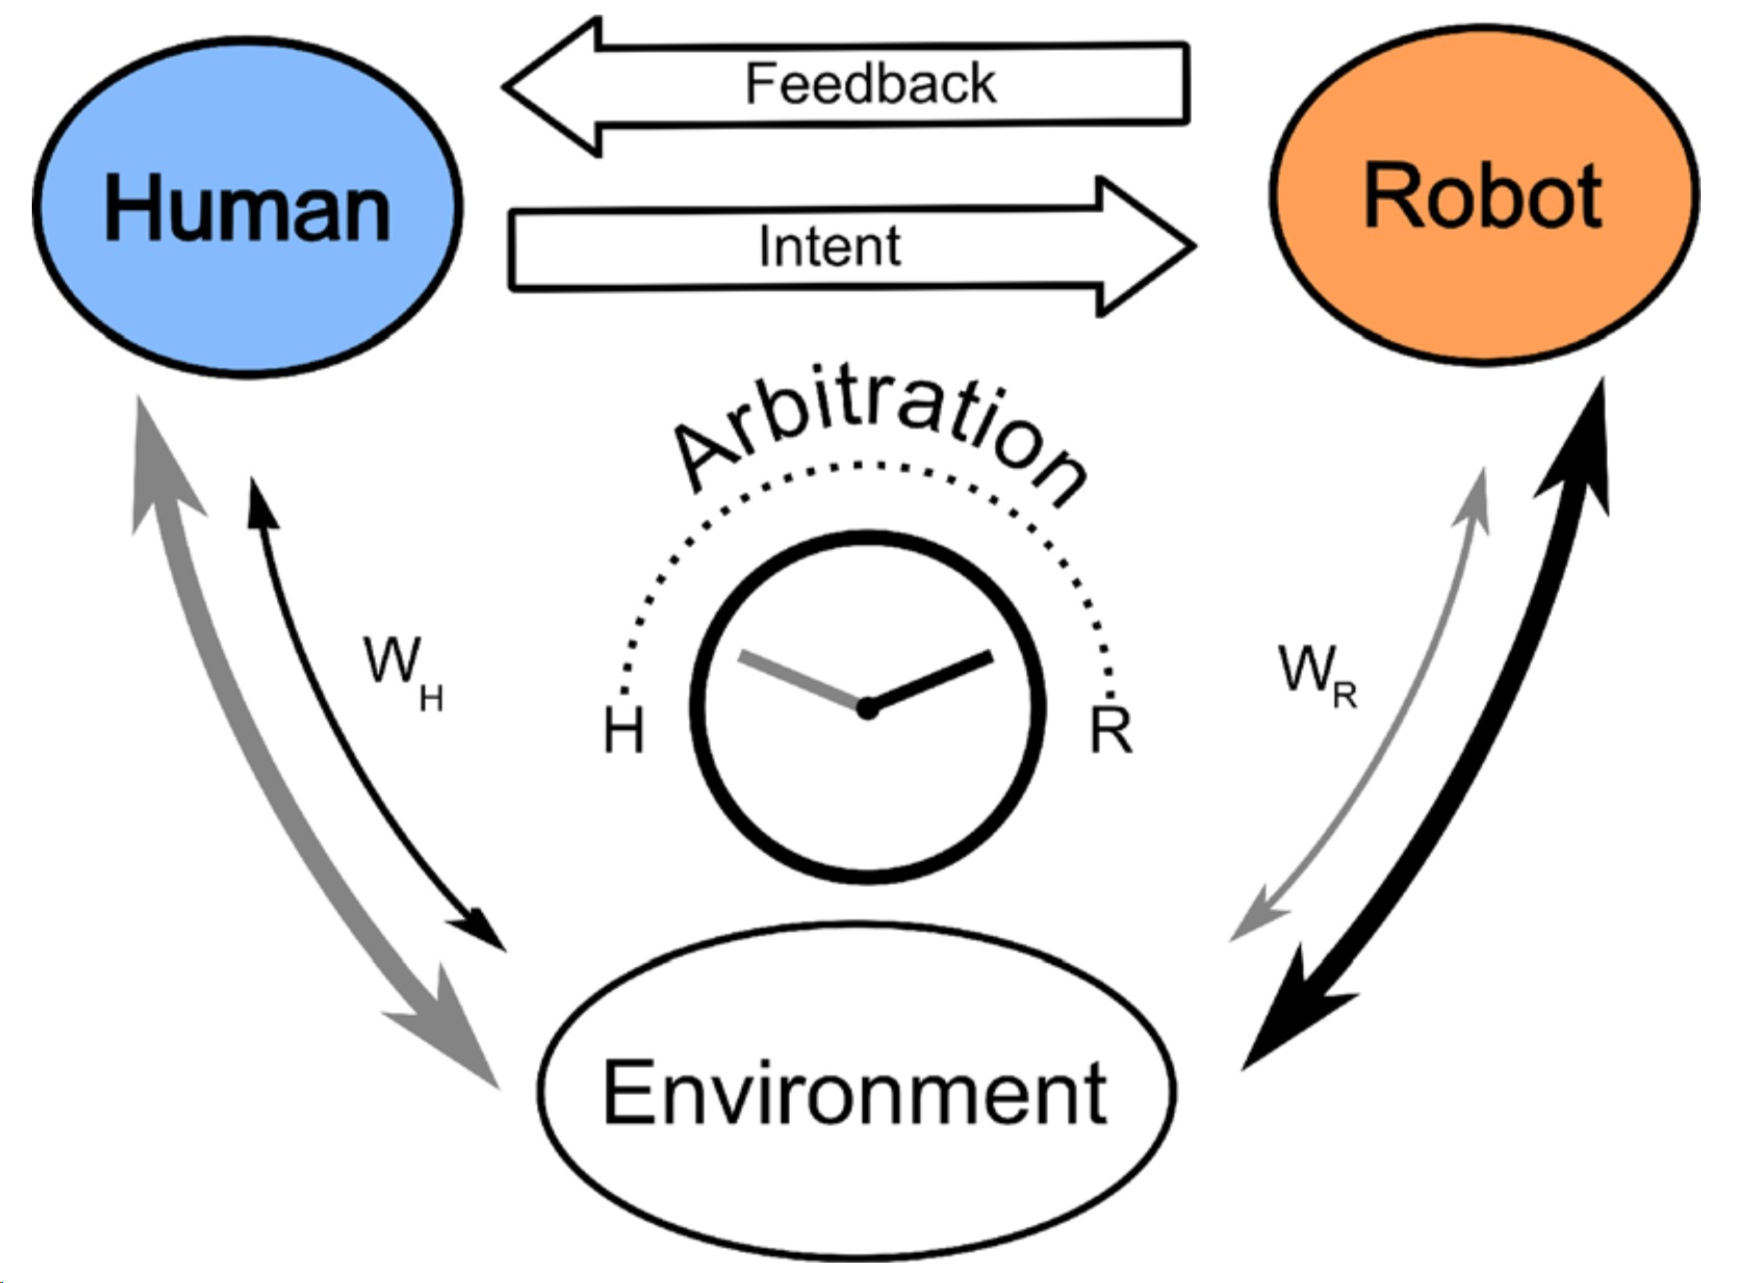
\includegraphics[width=0.8\linewidth]{figures/TradeStudy/figureb1.png}
%         \caption{Losey et al.'s proposed framework for human-robot interaction with the environment}
%         % \label{figure:}
%     \end{center}
% \end{figure}
% 	Losey et al.'s 2018 review discusses the state of the art in the field of physical human-robot interaction, where human abilities are enhanced or supported by robotic aids, and discuss the human factors involved with shared task execution between the human and robot. They present a unified view of shared human-robot control in physical task execution, using case studies of applications in healthcare to demonstrate their framework. Their framework focuses on three distinct phases of decision making: detection, the task of understanding the human's intent; arbitration, the task of distributing control between the human and robot; and feedback, the task of presenting the result of the human's intent, which is often done through haptic devices. One ongoing field of research in physical human-robot interaction is that of dynamic changes in role arbitration using machine learning and artificial intelligence techniques. The authors note role arbitration should re-evaluated when trust changes, and further note "robotic performance has the largest and most identifiable influence on trust in HRI." As such, the real-time monitoring of performance metrics is an area of active research.

% Wang, Tian-Miao, Yong Tao, and Hui Liu. "Current Researches and Future Development Trend of Intelligent Robot: A Review." International Journal of Automation and Computing (2018): 1-22.
% 	In their 2018 review, Wang et al. discuss current research and future development trends of "intelligent" robots. They note several key and leading technologies in the field of robotics. They include key technologies such as human-robot collaboration technology, autonomous navigation technology under non-structured environments, multi-agent robot systems (swarms), and emotion recognition and interaction mechanism of robot oriented to harmonious human-robot cooperation. They also highlight innovative leading technologies such as brain computer interfaces, brain-like robot control and decision making (artificial intelligence and supervised/unsupervised learning techniques), material cross-innovation and applications of robot oriented to software structure (3D printed materials, soft grippers, flexible robots), and network decision mechanism of robot based on cloud computing and big data (IoT, SLAM). Their review further breaks down these technology areas into more specific, individual technologies and notes the current state of the art in each.

\chapter{Aircraft Dynamics}

\section{Longitudinal Dynamics}
\begin{align*}
    \dot{\vec{x}}_{long} =
    \left[ \begin{array}{ *{5}{c} }
            X_u                     & X_w                     & X_q                                          & -g \cos \theta_0 & 0 \\
            Z_u                     & Z_w                     & Z_q + U_0                                    & -g \sin \theta_0 & 0 \\
            M_u + M_{\dot{w}} Z_{u} & M_w + M_{\dot{w}} Z_{w} & M_q + M_{\dot{w}} \left( Z_{q} + U_0 \right) & 0                & 0 \\
            0                       & 0                       & 1                                            & 0                & 0 \\
            0                       & -1                      & 0                                            & U_0              & 0 \\
        \end{array} \right]
    \left[ \begin{array}{ *{1}{c} }
            \Delta u      \\
            \Delta w      \\
            \Delta q      \\
            \Delta \theta \\
            \Delta z      \\
        \end{array} \right] & + \\
    \left[ \begin{array}{ *{5}{c} }
            X_{\delta_e}                            & X_{\delta_{th}}                               \\
            Z_{\delta_e}                            & Z_{\delta_{th}}                               \\
            M_{\delta_e} + M_{\dot{w}} Z_{\delta_e} & M_{\delta_{th}} + M_{\dot{w}} Z_{\delta_{th}} \\
            0                                       & 0                                             \\
            0                                       & 0                                             \\
        \end{array} \right]
    \left[ \begin{array}{ *{1}{c} }
            \Delta \delta_e    \\
            \Delta \delta_{th} \\
        \end{array} \right] &   \\
\end{align*}

\section{Lateral Dynamics}
\begin{align*}
    \dot{\vec{x}}_{lat} =
    \left[ \begin{array}{ *{5}{c} }
            Y_v  & Y_p  & Y_r - U_0     & g \cos \theta_0  & 0 \\
            L'_v & L'_p & L'_r          & -g \sin \theta_0 & 0 \\
            N'_v & N'_p & N'_r          & 0                & 0 \\
            0    & 1    & \tan \theta_0 & 0                & 0 \\
            0    & 0    & \sec \theta_0 & 0                & 0 \\
        \end{array} \right]
    \left[ \begin{array}{ *{1}{c} }
            \Delta v    \\
            \Delta p    \\
            \Delta r    \\
            \Delta \phi \\
            \Delta \psi \\
        \end{array} \right] & + \\
    \left[ \begin{array}{ *{5}{c} }
            Y_{\delta_{a}}  & Y_{\delta_{r}}  \\
            L'_{\delta_{a}} & L'_{\delta_{r}} \\
            N'_{\delta_{a}} & N'_{\delta_{r}} \\
            0               & 0               \\
            0               & 0               \\
        \end{array} \right]
    \left[ \begin{array}{ *{1}{c} }
            \Delta \delta_a \\
            \Delta \delta_r \\
        \end{array} \right] &   \\
\end{align*}



\end{document}
